% packages
\documentclass[12pt]{article}
\usepackage[utf8]{inputenc}
\usepackage[margin=1.1in]{geometry} % 0.9 for pset, 1.4 for livetex notes

% Math libraries
\usepackage{amsmath}
\usepackage{amssymb}
\usepackage{amsthm}
\usepackage{amsthm}

% Formatting
\usepackage{titling}
\usepackage{fancyhdr}
\usepackage{graphicx}
\usepackage{float}
\usepackage{titlesec}
\usepackage{setspace}
\usepackage[titles]{tocloft}

% Additional commands
\usepackage{cancel}
\usepackage{enumitem}
\usepackage{xfrac}
\usepackage{mathtools}

% Graphcs
\usepackage{tikz}
\usepackage{tcolorbox}
\usepackage{xcolor}
\usepackage{booktabs}
\usepackage{longtable}

% Content
\usepackage{physics}
\usepackage[version=4]{mhchem}
\usepackage{siunitx}
\usepackage{sectsty}

\allsectionsfont{\sffamily}
\renewcommand{\cftsecfont}{\normalfont\bfseries\sffamily}
\renewcommand*{\contentsname}{Table of Contents}

\newcommand*\circled[1]{\tikz[baseline=(char.base)]{
            \node[shape=circle,draw,inner sep=2pt] (char) {#1};}}
\renewcommand\real{\mathbb{R}}
\newcommand\complex{\mathbb{C}}
\newcommand\integer{\mathbb{Z}}
\newcommand\rational{\mathbb{Q}}
\newcommand\field{\mathbb{F}}
\newcommand\qsp{\qq{}}
\DeclarePairedDelimiter{\ceil}{\lceil}{\rceil}

\newcounter{lemmacounter}
\newcounter{definitioncounter}
\newtcolorbox{squarebox}{
  sharp corners,
  colback=blue!5!white,
  colframe=blue!75!black,
  boxrule=0.5px
}

\newtcolorbox{roundbox1}{
  colback=black!1!white,
  colframe=black!75!black,
  boxrule=0.5px
}

\newtcolorbox{roundbox2}{
  colback=yellow!5!white,
  colframe=red!75!black,
  boxrule=0.5px
}

% \newcounter{pblmcounter}
% \newenvironment{problem}
%   {\begin{boxedxx}
%   \stepcounter{pblmcounter}
%   \textbf{Statement of Problem}}
%   {\end{boxedxx}}
  
\newenvironment{solution}
  {\begin{proof}[Solution]}
  {\end{proof}}

\definecolor{DARKBLUE}{HTML}{005E7A}
\definecolor{BLACK}{HTML}{121212}
\definecolor{DARKRED}{HTML}{83223C}

\newenvironment{definition}
  {\begin{roundbox1}
  \stepcounter{lemmacounter}
  \textcolor{BLACK}{\textsf{\textbf{Definition \thesection.\arabic{lemmacounter}}}}}
  {\end{roundbox1}}

\newenvironment{example}
  {\begin{roundbox2}
  \stepcounter{lemmacounter}
  \textcolor{DARKRED}{\textsf{\textbf{Example \thesection.\arabic{lemmacounter}}}}}
  {\end{roundbox2}}

\newenvironment{lemma}
  {\begin{squarebox}
  \stepcounter{lemmacounter}
  \textcolor{DARKBLUE}{\textsf{\textbf{Lemma \thesection.\arabic{lemmacounter}}}}}
  {\end{squarebox}}
  
\newenvironment{theorem}
  {\begin{squarebox}
  \stepcounter{lemmacounter}
  \textcolor{DARKBLUE}{\textsf{\textbf{Theorem \thesection.\arabic{lemmacounter}}}}}
  {\end{squarebox}}
  
\newenvironment{proposition}
  {\begin{squarebox}
  \stepcounter{lemmacounter}
  \textcolor{DARKBLUE}{\textsf{\textbf{Proposition \thesection.\arabic{lemmacounter}}}}}
  {\end{squarebox}}

\makeatletter
\DeclareRobustCommand{\@seccntformat}[1]{%
  \def\temp@@a{#1}%
  \def\temp@@b{subsubsection}%
  \ifx\temp@@a\temp@@b
  \textcolor{DARKRED}{\csname the#1\endcsname}%
  \quad
  \else
  \textcolor{DARKBLUE}{§\csname the#1\endcsname}%
  \quad
  \fi
} 
\makeatother

\numberwithin{equation}{section}
\numberwithin{lemmacounter}{section}
\numberwithin{definitioncounter}{section}

\begin{document}
    \newcommand{\courseshort}{\textbf{Math 381}}
\newcommand{\coursetitle}{Fourier Analysis and Boundary Value Problems}
\newcommand{\term}{Fall Quarter 2023}

    \pagestyle{fancy}
    \fancyfoot[C]{}
    \fancyhead[L]{\textbf{Andrew Li} (\term)}
    \fancyfoot[L]{\courseshort \: \coursetitle}
    \fancyfoot[R]{\thepage}

    \title{\textbf{\textsf{\courseshort \, Lecture Notes}}}
    \author{Andrew Li}
    \date{\term}
    \clearpage\maketitle
    \noindent These are my original lecture notes for \textbf{Math 381: Fourier Analysis and Boundary Value Problems for ISP}, from Fall Quarter 2023, taught by Professor Nir Avni. I revised some of the formatting during Spring Quarter 2024, as this is the only math class I had taken notes live using \LaTeX, and could very well be the last. The $\varepsilon-\delta$ proofs in these notes, which were copied from what was done in lecture, are quite dubious and hard to follow. Further note that I omitted any examples from class from these notes, as they were generally quite trivial and straightforward, and I wanted to emphasize the proofs. That said, this document is still a valuable resource.
    \thispagestyle{empty}

    \tableofcontents
    \AddToHook{cmd/section/before}{\clearpage}
    
    \section{Lecture 1}
We can define STEM as subjects where we use Fourier Analysis.
\subsection{Some Motivation}
We can define the trajectory of a planet as the sum of $n$ cyclic motions
\begin{align}
    \vb{\gamma}(t) = \underset{\text{cycle}}{\vb{\gamma_1}(t)} + \underset{\text{epicycle}}{\vb{\gamma_2}(t)} + ... + \vb{\gamma_n}(t)
\end{align}
All functions can be approximated by the sum of many cyclic motions, which is Fourier analysis. In essence, Fourier analysis gives us a new way of thinking about functions.

\subsection{1D Example}
Suppose we have a linear cyclic motion; how can we make this with cycles? The sum of two vector functions
\begin{align}
    \vb{f}(t) &:= \langle \cos(t), \sin(t) \rangle\\
    \vb{g}(t) &:= \langle \cos(-t), \sin(-t) \rangle = \langle \cos(t), -\sin(t) \rangle \\
    \vb{h}(t) &:= \vb{f}(t) + \vb{g}(t) = \langle 2\cos(t), 0 \rangle
\end{align}

\subsection{Sets}
\begin{definition}
    A set is an unordered collection. There are many ways to specify a set:
    \begin{enumerate}
        \item As a group of a few elements:
        \begin{enumerate}
            \item $\{ 1, 2, 3 \}$
            \item $\{ 1, 2, 3, 4, 5 \}$
        \end{enumerate}
        \item As a group of a lot of elements:
        \begin{enumerate}
            \item $\{ 1, 2, 3, ..., 1000 \}$
            \item $\{ 1, 2, 3, ... \}$
        \end{enumerate}
        \item Using set builder notation:
        \begin{enumerate}
            \item $\{ x : \text{some condition for $x$} \}$
            \item $\{ n : n \text{ is the square of some integer $m$} \}$
        \end{enumerate}
    \end{enumerate}
\end{definition}
Sets are unordered, meaning
\begin{align}
    \{ 1, 2 \} = \{ 2, 1 \}
\end{align}
contrasting with sequences which are ordered, meaning
\begin{align}
    (1, 2) \ne (2, 1)
\end{align}
\subsubsection{Some common sets}
There are many common sets, such as
\begin{enumerate}
    \item $\mathbb{N}$ for natural numbers $\{ 0, 1, 2, 3, ... \}$
    \item $\mathbb{Z}$ for integers $\{ ..., -2, -1, 0, 1, 2, ... \}$
    \item $\mathbb{R}$ for real numbers
    \item $\mathbb{C}$ for complex numbers
\end{enumerate}
An element $n$ is said to be in a set $\mathbb{A}$, i.e. $n \in \mathbb{A}$, if $n$ is an element of $\mathbb{A}$. Note that $\in$ is not necessarily a statement of fact, so $\frac{1}{2}\in \mathbb{Z}$ is a perfectly valid statement; it's just false.

\subsection{Functions}
A function maps one set to another, not necessarily different set. For example,
\begin{align}
    f: \mathbb{A} \to \mathbb{B}
\end{align}
is a function mapping an input $x \in \mathbb{A}$ to an output $y \in \mathbb{B}$.
\subsection{Tuples}
A tuple, for example
\begin{align}
    (a_1, a_2, ..., a_n) && \text{n-tuple}
\end{align}
is actually a special kind of function
\begin{align}
    a: \{ 1, 2, ..., n \} \to \mathbb{A}
\end{align}
Each number in $\{ 1, 2, ..., n \}$ corresponds to a specific $a_i \in \mathbb{A}$.

\subsection{Complex Numbers}
The set of complex numbers is the set $\mathbb{C}$.
\begin{definition}
    Complex numbers are expressions of the form
    \begin{align}
        a + bi
    \end{align}
    where $a, b \in \mathbb{R}$ and $i := \sqrt{-1}$
\end{definition}
So, $\mathbb{C}$ can be expressed in set builder notation as
\begin{align}
    \mathbb{C} := \{ a+bi : a,b \in \mathbb{R} \}
\end{align}
From this there are two functions
\begin{align}
    \text{Re}: \mathbb{C} \to \mathbb{R} \Rightarrow \text{Re}(a+bi):=a\\
    \text{Im}: \mathbb{C} \to \mathbb{R} \Rightarrow \text{Im}(a+bi):=b
\end{align}
to take the real and imaginary components from a complex number. Further, define the conjugate of a complex number as
\begin{align}
    \overline{(a+bi)} := (a-bi)
\end{align}
Then,
\begin{align}
    (a+bi)\overline{(a+bi)} = a^2 + b^2
\end{align}
At a more fundamental level, this is true because $\mathbb{C}$ is a vector space, in which addition is defined through
\begin{align}
    (a+bi) + (c+di) := (a+c) + (b+d)i
\end{align}
and multiplication is defined through distribution:
\begin{align}
    (a+bi)(c+di) := ac + (ad + bc)i - bd
\end{align}
Finally, the absolute value of a complex number is defined as
\begin{align}
    |a + bi| := \sqrt{(a+bi)\overline{(a+bi)}}
\end{align}
Indeed, when $b=0$, $|a| = \sqrt{a^2}$, which is the same as for $\mathbb{R}$.
    \section{Lecture 2}
\subsection{A Continued Rant on Complex Numbers}
Think about $a+bi$ as the vector $\langle a, b \rangle$, giving complex numbers geometric significance. Hence, giving more motivation for (1.16). We can further write the inequalities
\begin{align}
    |\Im(z)|, |\Re(z)| \le |z| \le |\Im(z)| + |\Re(z)|
\end{align}
where $z \in \mathbb{C}$ per the triangle inequality.
\subsubsection{Dividing Complex Numbers}
We can divide complex numbers $z, w$ by multiplying the denominator by its conjugate:
\begin{align}
    \frac{z}{w} = \frac{z\overline{w}}{w \overline{w}}
\end{align}
as this will guarantee the denominator has no imaginary component per (1.15).

\subsection{A Discussion on Sequence Convergence}
What does it mean if a sequence of complex numbers converges?
\begin{definition}
    Let $z_1, z_2$ be a sequence of complex numbers, and let $w \in \mathbb{C}$. We can say that $\{ z_n \}$ converges to $w$, i.e.
    \begin{align}
        \lim_{n \to \infty}{z_n} = w
    \end{align}
    if
    \begin{align}
        \lim_{n \to \infty}{|z_n - w|} = 0
    \end{align}
\end{definition}
\begin{lemma}
\begin{align}
    z_n \to w \iff
    \begin{cases}
        \Re(z_n) \to \Re(w)\\
        \Im(z_n) \to \Im(w)
    \end{cases}
\end{align}
\end{lemma}
\begin{proof}
    From the triangle inequality for complex numbers,
    \begin{align}
        |z-w| \le |z|+|w|
    \end{align}
    It follows that $|z+w| \le |z|+|w|$. For $z\in\mathbb{C}$,
    \begin{align}
        |z|=|\Re(z)+i\Im(z)| \leq |\Re(z)|+|\Im(z)|
    \end{align}
    which we can convince ourselves of by drawing the complex number $z$ as a triangle, and using geometry to define each of these terms. Then,
    \begin{align}
        |z_n-z_\infty| \leq |\Re(z_n-z_\infty)|+|\Im(z_n-z_\infty)|
    \end{align}
    For $\Rightarrow$, we want to show
    \begin{align}
        z_n \to w \Rightarrow \begin{cases}
        \Re(z_n) \to \Re(w)\\
        \Im(z_n) \to \Im(w)
        \end{cases}
    \end{align}
    We can see this, as
    \begin{align}
        |z_n - w| &\le |\Re(z_n - w)| + |\Im(z_n - w)|\\
        &\le |\Re(z_n) - \Re(w)| + |\Im(z_n) - \Im(w)| \to 0\\
        &\Rightarrow |z_n - w| \to 0
    \end{align}
    noting that (2.11) is true via assumption. Then, for $\Leftarrow$ we want to show
    \begin{align}
        z_n \to w \Leftarrow \begin{cases}
        \Re(z_n) \to \Re(w)\\
        \Im(z_n) \to \Im(w)
        \end{cases}
    \end{align}
    Then,
    \begin{align}
        |\Re(z_n)-\Re(z_\infty)| \Rightarrow 0 && |\Im(z_n)-\Im(z_\infty)| \Rightarrow 0
    \end{align}
    which each imply
    \begin{align}
        |\Re(z_n-z_\infty)| \Rightarrow 0 && |\Im(z_n-z_\infty)| \Rightarrow 0
    \end{align}
    meaning, as $n \to \infty$, $|z_n - w| \le 0 \Rightarrow z_n \to w$.
\end{proof}

\subsection{Series Convergence}
\begin{definition}
    Let $z_1, z_2, ... \in \mathbb{C}$, and let $w \in \mathbb{C}$. We say that $\sum_{n=1}^\infty z_n \to w$ if $z_1, z_1 + z_2, ... \to w$
\end{definition}
\begin{lemma}
    Let $z_1, z_2, ...$ be a sequence of complex numbers. Assume that $\sum_{n=1}^\infty |z_n|$ converges, then $\sum_{n=1}^\infty z_n$ also converges. (This is called absolute convergence)
\end{lemma}
\begin{proof}
    Let $s_n := z_1 + ... + z_n$. We want to show that the sequence $s_n$ converges. We can show that $s_n$ converges by showing that both $\Re(s_n)$ and $\Im(s_n)$ converge. We know that
    \begin{align}
        \sum_{i=1}^n |\Re(z_i)| \le \sum_{i=1}^n |z_i|
    \end{align}
    because $|\Re(z)| \le |z|$ for all complex numbers $z \in \mathbb{C}$. By assumption, the latter converges, so 
    \begin{align}
        \sum_{i=1}^n |\Re(z_i)|
    \end{align}
    also must converge, meaning
    \begin{align}
        |\Re(s_n)|
    \end{align}
    converges. By the same reasoning,
    \begin{align}
        |\Im(s_n)|
    \end{align}
    converges, so $\sum_{n=1}^\infty z_n$ also converges.\footnote{Note from future self: this is a strange proof, but it works?}
\end{proof}

\subsection{Exponentials}
What is the meaning of $e^x$, or even $e^i$? We know that $e^x$ is a series
\begin{align}
    e^x = 1 + x + x^2/2 + x^3/6 + ... + x^n/n!
\end{align}
\begin{definition}
    For a complex number $z \in \mathbb{C}$, let $e^z$ be defined as
    \begin{align}
        e^z := \sum_{n=0}^\infty \frac{z^n}{n!}
    \end{align}
\end{definition}
This series converges because by Lemma 2.4, the sequence absolutely converges. We can look at
\begin{align}
    \sum |\frac{z^n}{n!}| = \sum \frac{|z^n|}{|n!|} = \sum \frac{|z|^n}{n!} = e^{|z|} < \infty
\end{align}
In general, suppose $t \in \mathbb{R}$. Then,
\begin{align}
    e^{it} = \sum_{n=0}^\infty \frac{(it)^n}{n!} = \text{the Taylor expansion goes here}
\end{align}
eventually we find
\begin{align}
    e^{it} = \cos(t) + i\sin(t)
\end{align}
by rearranging the Taylor expansion into even terms and odd terms.\footnote{Again, this seems like an awfully hand-wavy way to prove this. There is a better way to do the convergence proof, but this course did not do it.}
    \section{Lecture 3}
\subsection{Logarithms}
Logarithm was the most significant technological invention of the 16th century. The inverse, exponentials, also hold for $u \in \mathbb{C}$
\begin{align}
    e^{x+y} &= e^x \cdot e^y\\
    e^{it}\cdot e^{is} &= (\cos(t) + i\sin(t)) \cdot (\cos(s) + i\sin(s))\\
    &= (\cos(t)\cos(s) - \sin(t)\sin(t)) + i(\sin(t)\cos(s) + \cos(t)\sin(s))\\
    &= \cos(t+s) + i\sin(t+s)\\
    &= e^{i(t+s)}
\end{align}

\subsection{Calculus of Periodic Functions}
\begin{definition}
    $\mathbb{L} = \{ z \in \mathbb{C} \mid |z| = 1 \} = \{ e^{2\pi it} \}$
\end{definition}
\begin{lemma}
    The following types of functions are the same:
    \begin{enumerate}
        \item $f: \mathbb{R} \to \mathbb{C}$ that are periodic with period $1$
        \item $F: \mathbb{L} \to \mathbb{C}$
        \item $\Phi: [0, 1] \to \mathbb{C} \mid \Phi(0) = \Phi(1)$
    \end{enumerate}
\end{lemma}
Use the following
\begin{enumerate}
    \item Given $f: \mathbb{R} \to \mathbb{C}$, periodic with period $1$, let $F(e^{2\pi it}) = f(t)$  
    \item Given $f$,
    \begin{align}
        \Phi(x) := f(x)
    \end{align}
\end{enumerate}
Then we can take derivatives and integrals of these functions.
\subsubsection{Derivatives of functions $f: \mathbb{R} \to \mathbb{C}$}
A function into $\mathbb{C}$ is effectively a pair of two functions, $f_\text{Re} (t): \mathbb{R} \to \mathbb{R}$ and $f_\text{Im} (t): \mathbb{R} \to \mathbb{R}$. Then, define
\begin{align}
    f'(t) &:= f'_\text{Re}(t) + i f'_\text{Im}(t)\\
    \int f(t) \dd{t} &:= \int f'_\text{Re}(t)\dd{t} + i \int f'_\text{Im}(t)\dd{t}
\end{align}
We can use these to prove that the product rule, quotient rule, derivative rules, integration by parts, etc. all work the same for $\mathbb{C}$.\footnote{It would have been better to frame these explicitly as vectors, and differentiation/integration as linear transformations, but that did not happen.}

\subsection{Vector Spaces}
\begin{definition}
    A real vector space is a set $V$ whose elements (vectors) $\vb{v}$, with two operations:
    \begin{enumerate}
        \item Closedness under addition $\vb{v_1} + \vb{v_2} \in V$
        \item Closedness under scalar multiplication $c\vb{v} \in V$
    \end{enumerate}
    such that the other rules for vector spaces are satisfied\footnote{See Axler \textit{Linear Algebra Done Right}}.
\end{definition}
Niche but interesting examples
\begin{enumerate}
    \item $C_\mathbb{R}[0,1] := \{ f: [0,1] \to \mathbb{R} \mid f \text{ is continuous}\} := (3.3.1)$
    \item $\{ f: [0,1] \to \mathbb{R} \mid f \text{ has finitely many discontinuities}\} := (3.3.2)$
\end{enumerate}
Note that $(3.3.1) \subseteq (3.3.2)$.
    \section{Lecture 4}
\subsection{More on Derivatives and Integrals}
Derivatives represent position, velocity, acceleration, jerk, etc.
\begin{align}
    \dv{}{t} \left(e^{it} \right) = ie^{it}
\end{align}
This is the velocity of the trajectory and multiplying by $i$ induces a $90^\circ$ rotation. Integrals then might represent the center of mass, or more generally, a complete sum which can be used for averages.
\begin{lemma}
    \begin{align}
        \int_0^{2\pi} e^{int}e^{-imt} \dd{t} = \begin{cases}
            0 \implies n\ne m\\
            2\pi \text{ otherwise}
        \end{cases}
    \end{align}
\end{lemma}

\subsection{Inner Product}
The dot product in $\mathbb{R}^n$ is denoted by
\begin{align}
    (x_1, x_2, ..., x_n) \cdot (y_1, y_2, ..., y_n) = \sum_{i=1}^n x_iy_i
\end{align}
For functions, this does not quite work, as there are infinitely many terms; instead, an integral is a better tool to represent the inner product.
\begin{definition}
    The standard inner product on $C_\mathbb{R}[0,1]$ is the function that takes two vectors $f, g \in C_\mathbb{R}[0,1]$ and outputs the number
    \begin{align}
        \langle f, g \rangle := \int_0^1 f(x)g(x) \dd{x}
    \end{align}
\end{definition}
This is the ``infinite dimensional version of the dot product'' and satisfies many of the same properties:
\subsubsection{Properties of a (Real) Inner Product}
\begin{definition}
    Any real inner product satisfies:
    \begin{enumerate}
        \item $\langle f, g \rangle = \langle g, f \rangle$
        \item $\langle \lambda f, g \rangle = \lambda \langle f, g \rangle$
        \item $\langle f + g, h \rangle = \langle f, h \rangle + \langle g, h \rangle$
        \item $\langle f, f \rangle \ge 0$
        \begin{enumerate}
            \item $\langle f, f \rangle = 0 \iff f = 0$
        \end{enumerate}
    \end{enumerate}
\end{definition}
\textbf{Any function that satisfies these four properties is an inner product.} With these we can also talk about length and angle.
\begin{definition}
    If $f, g \in V$\footnote{a vector space}, define the norm of $f$ as
    \begin{align}
        \norm{f} := \sqrt{\langle f, f \rangle}
     \end{align}
     Then, the distance between $f$ and $g$ is $\norm{f-g}$ and the angle between them is the number $\gamma$ such that
     \begin{align}
         \langle f, g \rangle = \norm{f} \cdot \norm{g} \cdot \cos(\gamma)
     \end{align}
     Finally, if the angle between $f$ and $g$ is $\pi/2$ radians, then we say that $f \perp g$ (the inner product must be zero).
\end{definition}
    \section{Lecture 5}
Complex functions/numbers form a complex vector space, such as $\mathbb{C}^2$. 
\subsection{Complex Inner Products}
Inner products are weirder in the complex case, as
\begin{align}
    \langle if, if \rangle = -1 \langle f, f \rangle
\end{align}
What changes is that
\begin{align}
    \langle f, g \rangle = \langle g, f \rangle
\end{align}
is no longer true.
\begin{definition}
    Let $V$ be a complex vector space. An inner product on $V$ is a function that takes two vectors $\vb{u}, \vb{v} \in V$ and outputs $\langle v, u \rangle \in \mathbb{C}$.
\end{definition}
\subsection{Properties of a (Complex) Inner Product}
\begin{definition}
    Any complex inner product satisfies:
    \begin{enumerate}
        \item $\langle u, v \rangle = \overline{\langle v, u \rangle}$
        \item $\langle \lambda u, v \rangle = \lambda \langle u, v \rangle$
        \item $\langle u + v, w \rangle = \langle u, w \rangle + \langle v, w \rangle$
        \item $\langle u, u \rangle \ge 0$
        \begin{enumerate}
            \item $\langle u, u \rangle = 0 \iff u = 0$
        \end{enumerate}
    \end{enumerate}
\end{definition}
Note that
\begin{align}
    \langle v, \lambda w \rangle \ne \lambda \langle v, w \rangle
\end{align}
but we can combine rules to find
\begin{align}
    \langle v, \lambda w \rangle &= \overline{
        \langle \lambda w, v \rangle
    }\\
    &= ... = \overline{\lambda} \cdot \langle v, w \rangle
\end{align}
Then, as an example
\begin{align}
    C[0,1] := \{ f: [0,1] \to \mathbb{C} \mid f \text{ continuous} \}
\end{align}
This is a complex vector space.
\begin{definition}
    The standard inner product on $C[0,1]$ is
    \begin{align}
        \langle f, g \rangle = \int_0^1 \left[ f(t) \overline{g(t)} \right] \dd{t}
    \end{align}
\end{definition}

\subsection{Fourier Motivation}
Given
\begin{align}
    f(t) = \alpha_0 e^{\beta_0 i t} + \alpha_1 e^{\beta_1 i t} + \alpha_2 e^{\beta_2 i t} + ...
\end{align}
How can we find $\alpha$? Using this integral
\begin{align}
    \int_0^1 \left[ e^{2\pi int} \cdot e^{-2\pi imt} \right] \dd{t} = \begin{cases}
        1 & n = m\\
        0 & n \ne m
    \end{cases}
\end{align}
This is just an inner product using (5.7):
\begin{align}
    \langle e^{2\pi i n t}, e^{2\pi i m t} \rangle
\end{align}
We can quite easily find what $\alpha$ are:
\begin{align}
    \langle f(t), e^{\beta_1 i t} \rangle = ... = \alpha_1
\end{align}
via linearity of the inner product. Using (5.9), all terms cancel except that for $\alpha_1$. So, taking the integral gives that constant.
\begin{definition}
    A set $\{ \vb{v_i} \}$ of vectors in a vector space with an inner product is orthonormal\footnote{orthogonal and normalized} if
    \begin{enumerate}
        \item Orthogonal $\langle \vb{v_i}, \vb{v_j} \rangle = 0 \iff i \ne j$
        \item Normalized $\langle \vb{v_i}, \vb{v_i} \rangle = 1$
    \end{enumerate}
\end{definition}
Then, it follows that
\begin{lemma}
    If $\vb{v_1}, ... \vb{v_n}$ are orthonormal and $\vb{v} = \alpha_1\vb{v_1} + ... + \alpha_n\vb{v_n}$ then
    \begin{align}
        \alpha_i = \langle \vb{v}, \vb{v_i} \rangle
    \end{align}
\end{lemma}
In general, there are two definitions to take away from this
\begin{definition}
    \begin{enumerate}
        \item If $\{ \vb{v_i} \}$ are orthonormal, $\vb{v} \in V$, the numbers $\langle \vb{v}, \vb{v_i} \rangle$ are called the generalized Fourier coefficients of $\vb{v}$.
        \item If $\{ \vb{v_1}, ... \vb{v_n}  \}$ are orthonormal, $v \in V$, the vector
        \begin{align}
            P_{\{ \vb{v_1}, ... \vb{v_n} \}} \vb{v} := \langle \vb{v}, \vb{v_1} \rangle \vb{v_1} + ... + \langle \vb{v}, \vb{v_n} \rangle \vb{v_n}
        \end{align}
        is called the projection of $v$.
    \end{enumerate}
\end{definition}
But what if $v$ is not an element of $V$?
\begin{lemma}
    Assume $\{ v_1,...,v_n \}$ are orthonormal, $v \in V$. Then:
    \begin{enumerate}
        \item $\vb{v} - P\vb{v}$ is orthogonal to any linear combination of $\vb{v_1}, ... \vb{v_n}$
        \item For every $\vb{w} \in W$, $\norm{\vb{u} - \vb{w}}^2 = \norm{\vb{u} - P_W\vb{u}}^2 + \norm{P_W \vb{u} - \vb{w}}^2$
        \item Among all vectors that are linear combinations of $\vb{v_1}, ... \vb{v_n}$, $P\vb{v}$ is the closest to $\vb{v}$ 
        \item Let $\{ \vb{v_i} \}$ be orthonormal vectors in an inner product space $V$, and let $\vb{v} \in V$. Then,
        \begin{align}
            \sum \abs{\langle \vb{v}, \vb{e_i} \rangle}^2 \le \norm{\vb{v}}^2
        \end{align}
    \end{enumerate}
\end{lemma}
\begin{enumerate}
    \item \begin{proof}
        Suppose $\vb{w}$ is some linear combination of $\{ v_1,...,v_n \}$. Then,
        \begin{align}
            \langle P\vb{v}, \vb{v_i} \rangle
            &= 
                \left\langle
                    \left[\langle \vb{v}, \vb{v_1} \rangle \vb{v_1} + ... + \langle \vb{v}, \vb{v_n} \rangle \vb{v_n}\right], \vb{v_i} 
                \right\rangle\\
            &= \left\langle \langle \vb{v}, \vb{v_1} \rangle \vb{v_1}, \vb{v_i} \right\rangle + ... + \left\langle \langle \vb{v}, \vb{v_n} \rangle \vb{v_n}, \vb{v_i} \right\rangle\\
            &= \left\langle \langle \vb{v}, \vb{v_i} \rangle \vb{v_i}, \vb{v_i} \right\rangle\\
            &= \langle \vb{v}, \vb{v_i} \rangle \left\langle \vb{v_i}, \vb{v_i} \right\rangle = \langle \vb{v}, \vb{v_i} \rangle && \left\langle \vb{v_i}, \vb{v_i} \right\rangle = 1\\
            \implies& \langle P\vb{v} - \vb{v}, \vb{w} \rangle = 0
        \end{align}
    \end{proof}
    \item \begin{proof}
        \begin{align}
            \norm{\vb{u} - \vb{w}}^2 &= \norm{(\vb{u} - P_W\vb{u}) + (P_W\vb{u} - \vb{w})}^2\\
            &= \norm{\vb{u} - P_W\vb{u}}^2 + \norm{P_W\vb{u} - \vb{w}}^2 && \text{(5.19) $\implies$ orth.}
        \end{align}
    \end{proof}
    \item \begin{proof}
        Suppose $\vb{w}$ is a linear combination of $\{ \vb{v_1},...,\vb{v_n} \}$. WTS $\norm{\vb{w} - \vb{v}} > \norm{P\vb{v} - \vb{v}}$.
        \begin{align}
            \norm{\vb{w}-\vb{v}}^2 &= \norm{(\vb{w}-P\vb{v}) + (P\vb{v} - \vb{v})}^2 && \text{use orth.}\\
            &= \norm{\vb{w}-P\vb{v}}^2 + \norm{P\vb{v} - \vb{v}}^2 \ge \norm{P\vb{v} - \vb{v}}^2 && \text{term 1 $\ge$ 0}
        \end{align}
    \end{proof}
    \item \begin{proof}
        \begin{align}
            \norm{\vb{u}}^2 &= \norm{\vb{u} - P_W\vb{u}}^2 + \norm{P_W\vb{u}}^2 && (5.21)\\
            &\ge \norm{P_W\vb{u}}^2 = \norm{\langle \vb{u}, \vb{v_1} \rangle \vb{v_1} + ... + \langle \vb{u}, \vb{v_n} \rangle \vb{v_n}}^2 && \ge 0\\
            &\ge \norm{\langle \vb{u}, \vb{v_1} \rangle \vb{v_1}}^2 + \norm{\langle \vb{u}, \vb{v_2} \rangle \vb{v_2}}^2 + ... + \norm{\langle \vb{u}, \vb{v_n} \rangle \vb{v_n}}^2 && \text{orth.}\\
            &\ge \abs{\langle \vb{u}, \vb{v_1} \rangle}^2 + ... + \abs{\langle \vb{u}, \vb{v_2} \rangle}^2 + ... + \abs{\langle \vb{u}, \vb{v_n} \rangle}^2 && \text{norm.}\\
            & \ge \sum \abs{\langle \vb{v}, \vb{e_i} \rangle}^2
        \end{align}
        So flip the inequality to complete the proof
        \begin{align}
            \sum \abs{\langle \vb{v}, \vb{e_i} \rangle}^2 \le \norm{\vb{u}}^2
        \end{align}
    \end{proof}
\end{enumerate}
    \section{Lecture 6}
\subsection{Convergence}
Instead of convergence of points, convergence of functions, which is the reason infinite dimensional vector spaces are important.
\subsection{Tangent: Triangle Inequality and Cauchy-Schwartz}
\begin{definition}
If $V$ is a vector space with an inner product, and $\vb{u}, \vb{v} \in V$, then
\begin{align}
    \norm{\vb{u} + \vb{v}} \le \norm{\vb{u}} + \norm{\vb{v}}
\end{align}
\end{definition}
\begin{definition}
    Cauchy-Schwartz Inequality\footnote{It's quite odd that this was framed as a definition in lecture, but I will leave it as is.}
    \begin{align}
        \abs{\langle \vb{u}, \vb{v} \rangle} \le \norm{\vb{u}}\norm{\vb{v}}
    \end{align}
    \begin{proof}
        In the real case,
        \begin{align}
            f(t) :=& \norm{\vb{u} + t\vb{v}}^2 = \langle \vb{u} + t\vb{v}, \vb{u} + t\vb{v} \rangle\\
            =& \norm{\vb{u}}^2 + 2t \langle \vb{u}, \vb{v} \rangle + t^2 \norm{\vb{v}}^2 \ge 0\\
            \implies & \text{$\Delta \le 0$} & \text{1 sol. or 0 sol.}\\
            \implies & 4\langle \vb{u}, \vb{v} \rangle ^2 - 4\norm{\vb{u}}^2\norm{\vb{v}}^2 \le 0\\
            \implies & \langle \vb{u}, \vb{v} \rangle ^2 \le \norm{\vb{u}}^2\norm{\vb{v}}^2
        \end{align}
    \end{proof}
\end{definition}

\subsection{Back to Convergence}
\begin{definition}
    Let $V$ be a vector space with an inner product. Let $\vb{v}_1, \vb{v}_2, ...$ be a sequence of vectors. We say
    \begin{align}
        &\lim_{n\to\infty} \vb{v}_n = \vb{v}_\infty \impliedby \lim_{n\to\infty} \norm{\vb{v}_n - \vb{v}_\infty} = 0\\
        &\sum_1^\infty \vb{v}_n = \vb{w} \impliedby \vb{v}_1, \vb{v}_1 + \vb{v}_2, ..., \vb{v}_1 + \vb{v}_2 + ... + \vb{v}_n \to \vb{w}
    \end{align}
\end{definition}
\begin{lemma}
    If $\vb{v}_n \to \vb{v}_\infty$, then $\norm{\vb{v}_n} \to \norm{\vb{v}_\infty}$
\end{lemma}
\begin{proof}
    Apply $\Delta$ inequality to $\vb{v}_\infty$ and $\vb{v}_n - \vb{v}_\infty$. So
    \begin{align}
        \norm{\vb{v}_n} \le \norm{\vb{v}_\infty} + \norm{\vb{v}_n - \vb{v}_\infty}
    \end{align}
    Take limit of both sides and
    \begin{align}
        \lim \norm{\vb{v}_n} \le \norm{\vb{v}_\infty} + \lim \norm{\vb{v}_n - \vb{v}_\infty}
    \end{align}
    We can then apply the $\Delta$ inequality the other way and we get
    \begin{align}
        &\norm{\vb{v}_\infty} \le  \lim \norm{\vb{v}_n} + \lim \norm{\vb{v}_\infty - \vb{v}_n}
    \end{align}
    \begin{align}
&\boxed{            \norm{\vb{v}_\infty} \le \lim \norm{\vb{v}_n} \le \norm{\vb{v}_\infty}
\implies            \lim \norm{\vb{v}_n} = \norm{\vb{v}_\infty}}
    \end{align}
\end{proof}

\begin{definition}
    Suppose $\{ \vb{v}_n \}$ is an orthonormal sequence in $V$. We say that $\{ \vb{v}_n \}$ is closed (or that they are an orthonormal basis) if for every $\vb{v} \in V$,
    \begin{align}
        \vb{v} = \sum_{i=1}^\infty \langle \vb{v}, \vb{v}_i \rangle \vb{v}_i
    \end{align}
\end{definition}

\subsection{Main Theorem of This Course}
\begin{theorem}
    The set
    \begin{align}
        \{ e^{2\pi int} \}
    \end{align}
    forms a closed, orthonormal set of functions in $C[0,1]$.
\end{theorem}

    \section{Lecture 7}
\subsection{Fourier Series for Real Functions}
Suppose $f: [0,1] \to \mathbb{R}$. Fourier analysis of this function says,
\begin{align}
    f(t) = \sum_{n \in \mathbb{Z}} a_n e^{2\pi int} \mid a_n = \left\langle f(t), e^{2\pi int} \right\rangle
\end{align}
Since this is a real function, we can establish
\begin{lemma}
    For real function $f: [0,1] \to \mathbb{R}$
    \begin{align}
        \overline{a_n} = a_{-n} \mid a_n = \left\langle f(t), e^{2\pi int} \right\rangle
    \end{align}
\end{lemma}
\begin{proof}
    \begin{align*}
        a_n &= \int_0^1 f(t) \overline{e^{2\pi int}} \dd{t}\\
        \overline{a_n} &= \overline{\int_0^1 f(t) \overline{e^{2\pi int}} \dd{t}} = \int_0^1 \overline{f(t) \overline{e^{2\pi int}}} \dd{t}\\
        &= \int_0^1 \overline{f(t)} e^{2\pi int} \dd{t}\\
        &= \int_0^1 f(t) e^{2\pi int} \dd{t} & f(t) \in \mathbb{R}\\
        &= \int_0^1 f(t) \overline{e^{-2\pi int}} \dd{t} = \left\langle f(t), e^{-2\pi int} \right\rangle = a_{-n}
    \end{align*}
\end{proof}
\noindent Using Lemma 7.1,
\begin{align}
    f(t) &= a_0 + \sum_{n > 0} a_n e^{2\pi int} + a_n e^{-2\pi int}\\
    &= a_0 + \sum_{n > 0} a_n e^{2\pi int} + a_n \overline{e^{2\pi int}}
\end{align}
Then, using the radial complex form
\begin{align}
    a_n = r_n \cdot e^{i\theta_n}
\end{align}
where $r_n$ is the radius of the complex vector and $\theta_n$ is its angle relative to $\langle 1, 0\rangle$,
\begin{align}
    f(t) &= a_0 + \sum r_n \left[ e^{2\pi int + i\theta_n} + e^{2\pi int - i\theta_n} \right] & \text{second term uses $-n$}
\end{align}
We are adding a complex number and its conjugate\footnote{$(a + bi) + (a - bi) = 2a$}, so
\begin{align}
    \boxed{f(n) = a_0 + \sum_{n=1}^\infty 2r_n \cos\left[ 2\pi nt + \theta_n \right]}
\end{align}
proving that all real functions can be composed as the sum of trigonometric functions.

\subsection{Digression on Sound}
A sound is some function
\begin{align}
    f(n) = \sum_n a_n e^{2\pi int}
\end{align}
But humans can only hear certain frequencies so the function
\begin{align}
    f(n) = \sum_n^{20000} a_n e^{2\pi int}
\end{align}
sounds the same. We thus only need 40000 numbers $-20000, -19999, ..., 19999, 20000$ to represent a sound at some time $t$ (in order to use 7.7 we need to cancel the exponential).
\subsubsection{Sound Compression}
\texttt{mp3} compression algorithms pick the top $n$ frequencies at a certain time and delete the rest, saving space. On top of this, harmonic analysis can be performed to determine which frequencies are ``cancelled out'' and remove them too, further saving space.

    \section{Lecture 8}
\subsection{Bessel and Parseval}
\begin{lemma}
    Let $V$ be a vector space with an inner product; let $v_1, v_2, ... \in V$ be an orthonormal set. Then, let $v \in V$. Then,
    \begin{enumerate}
        \item (Bessel's Inequality)
        $$\norm{v}^2 \ge \sum_i^{N \le \dim V} \abs{\langle v, v_i \rangle}^2$$
        \item (Parseval's Theorem) If $\{ v_i \}$ is complete, then
        $$\norm{v}^2 = \sum_i^{\dim V} \abs{\langle v, v_i \rangle}^2$$
    \end{enumerate}
\end{lemma}
\begin{proof}
    From Lemma 5.7,
    \begin{align}
        (v - P_Wv) \perp w \mid \forall w \in W:= \text{span} \{v_1, v_2, ..., v_N\} \mid \forall N \in \mathbb{Z}
    \end{align}
    So, $(v - P_Wv) \perp P_W v$. Then, by the Pythagorean Theorem,
    \begin{align}
        \norm{v}^2 &= \norm{P_Wv}^2 + \norm{v - P_Wv}^2 \ge \norm{P_Wv}^2\\
        \implies \norm{v}^2 &\ge \norm{P_Wv}^2
    \end{align}
    So, recall (5.13), and write the right side as
    \begin{align}
        \left\langle \sum_{i=1}^N \langle v, v_i \rangle v_i, \sum_{j=1}^N \langle v, v_j \rangle v_j \right\rangle
    \end{align}
    But, when $i \ne j$, this goes to $0$ due to orthonormality. So,
    \begin{align}
        (8.5) &= \left\langle \sum_{i=1}^N \langle v, v_i \rangle v_i, \sum_{i=1}^N \langle v, v_i \rangle v_j \right\rangle\\
        &= \sum_{i=1}^N \langle v, v_i \rangle \overline{\langle v, v_i \rangle} = \sum_{i=1}^N \abs{\langle v, v_i \rangle}^2
    \end{align}
    Thus, 
    \begin{align}
        \norm{v}^2 &\ge (\norm{P_Wv}^2 = \sum_{i=1}^N \abs{\langle v, v_i \rangle}^2 )\\
        \implies \norm{v}^2 &\ge \sum_{i=1}^N \abs{\langle v, v_i \rangle}^2
    \end{align}
    In particular, as $N \to \infty$,
    \begin{align}
        \norm{v}^2 &= \sum_{i=1}^\infty \abs{\langle v, v_i \rangle}^2
    \end{align}
    Recall that we assume that $\{ v \}$ is complete. So, by definition,
    \begin{align}
        v = \lim_{N \to \infty} P_W v
    \end{align}
    that is, these approximations converge back to $v$ as $W \to \text{ completeness}$. By Lemma 6.4,
    \begin{align}
        \lim_{N \to \infty} \norm{P_W v} \to \norm{v}
    \end{align}
    so
    \begin{align}
        \lim_{N \to \infty} \norm{P_W v}^2 \to \norm{v}^2
    \end{align}
    which becomes, by (8.8),
    \begin{align}
        \lim_{N \to \infty} \sum_{i=1}^N \abs{\langle v, v_i \rangle}^2 &\to \norm{v}^2\\
        \implies \norm{v^2} &= \sum_{i=1}^\infty \abs{\langle v, v_i \rangle}^2
    \end{align}
\end{proof}

\subsection{An Example}
Let
\begin{align}
    V = C[0,1] \mid \{ e^{2\pi int} \} \text{ be complete}
\end{align}
We use the second simplest function\footnote{What is the first simplest function?!}
\begin{align}
    v = t
\end{align}
By Bessel,
\begin{align}
    \norm{t}^2 = \sum \abs{\langle t, e^{2\pi int} \rangle}^2
\end{align}
We take the inside and evaluate it
\begin{align}
    \langle t, e^{2\pi int} \rangle = \int_0^1 t \cdot e^{2\pi int} \dd{t}
\end{align}
and by parts it into\footnote{This is not AP Calculus AB so the proof is not going to be copied into these notes.}
\begin{align}
    \dfrac{-1}{2\pi in}
\end{align}
The edge case is at $n=0$, which when we plug into (8.18) yields $\frac{1}{2}$. The left hand side of (8.17) is $\frac{1}{3}$. So,
\begin{align}
    \frac{1}{3} &= (\frac{1}{2})^2 + 2\sum_{n=1}^\infty \frac{1}{4\pi^2 n^2}\\
    \frac{1}{6} &= \sum \frac{1}{\pi^2 n^2}\\
    \frac{\pi^2}{6} &= \sum \frac{1}{n^2}
\end{align}
    \section{Lecture 9}
``This is the beginning of the analysis part of this course''
\subsection{The Notion of Convergence}
There are three competing schools of thought when it comes to convergence
\begin{definition}
    Let $f_n(x), g(x) \in C^\mathbb{C}[0,1]$. Then, we say
    \begin{enumerate}
        \item If $\norm{f_n(x) - g(x)} \to_{n\to\infty} 0$, then we say $f_n(x)$ \textbf{converges in norm} to $g(x)$
        \item If $\forall a, \forall \varepsilon > 0$, $\exists N$ such that
        $$\forall n > N \implies \abs{f_n(a) - g(a)} < \varepsilon$$
        then we say $f_n(x)$ \textbf{converges pointwise} to $g(x)$
        \item If $\forall \varepsilon > 0$, $\exists N$ such that
        \begin{align}
            \begin{cases}
                \forall a \in [0,1]\\
                \forall n > N
            \end{cases}
            \implies \abs{f_n(a) - g(a)} < \varepsilon
        \end{align}
        then we say $f_n(x)$ \textbf{converges uniformly} to $g(x)$
    \end{enumerate}
\end{definition}
Then, we claim that
\begin{proposition}
    For continuous $n$-differentiable functions $f_n$, the Fourier approximations of $f_n$ converge pointwise to $f_n$.
\end{proposition}
First, prove a Lemma
\begin{lemma}
    Suppose $f: [0,1] \to \mathbb{C}$ is continuous. Then,
    \begin{align}
        \braket{f}{e^{2\pi int}} \to_{n\to\infty} 0
    \end{align}
\end{lemma}
\begin{proof}
    Use Bessel's Inequality
    \begin{align}
        \forall N, \sum_{n=-N}^N \abs{\braket{f}{e^{2\pi int}}}^2 &= \norm{P_{\{e^{-2\pi iNt}, \dots, e^{2\pi int}\}}f}^2\\
        &= \norm{f_N}^2\\
        &\le \norm{f}^2
    \end{align}
    so as to say for all $N$, this sum is \textbf{bounded}. So, taking $N \to \infty$,
    \begin{align}
        \lim_{N\to\infty} \sum_{n=-N}^N \abs{\braket{f}{e^{2\pi int}}}^2  \begin{cases}
            \text{converges}\\
            \text{diverges ($\to \infty$)}
        \end{cases}
    \end{align}
    but, divergence is impossible by (9.5), as this sum is \textbf{bounded}, so the individual terms must $\to 0$ in order to converge.
\end{proof}
Now we can establish a major theorem.
\begin{theorem}
    Suppose $f: \mathbb{R} \to \mathbb{C}$ is some periodic function of period $1$ and is continuous and differentiable. Let $S_n$ be the $n$th partial Fourier expansion of $f$.
    \begin{align}
        (S_Nf)(x) = \sum_{n=-N}^N \braket{f}{e^{2\pi int}} \cdot e^{2\pi int}
    \end{align}
    Then, we claim
    \begin{align}
        (S_Nf) \to f \qq{pointwise}
    \end{align}
\end{theorem}
\begin{proof}
    We can first prove this for $f(x) = 1$:
    \begin{align}
        (S_Nf)(0) = \sum_{n=-N}^N \braket{1}{e^{2\pi int}} \cdot 1 = 1
    \end{align}
    and we claim that extending this theorem for all $f \in \mathcal{F} \mid f(0) = 0$ is enough to prove that this theorem applies to all functions $g(x)$:
    \begin{align}
        \begin{cases}
            g(0) = 0 \to \text{cool}\\
            g(0) \ne 0 \to \text{define } h(x) := g(x) - g(0)
        \end{cases}
    \end{align}
    and we know this works because this forces $g(0) = 0$. We can prove this:
    \begin{align}
        (S_Nh) \stackrel{?}{\to} h\\
    \end{align}
    This is trivial because we can use the linearity of $S_N$ which is (clearly) a linear transformation
    \begin{align}
        S_Nh &= S_N(g(x) - g(0))\\
        &= S_Ng - S_N(g(0))\\
        &= S_Ng - g(0)\cdot S_N(1)\\
        &= S_Ng - g(0)
    \end{align}
    If we can show $S_Ng \to g$, then (9.16) is trivially true by (9.10B)
    \begin{lemma}
        The claim $S_Ng \to g$, is true for $x = 0$.
    \end{lemma}
    \begin{proof}
        \begin{align}
            (S_Nf)(0) &= \sum_{n=-N}^N \left[ \int_0^1 f(t) e^{-2\pi int} \dd{t} \right] \cdot e^{2\pi in(0)}\\
            &= \int_0^1 f(t) \sum_{n=-N}^N e^{-2\pi int} \dd{t}\\
            &= \int_0^1 f(t) \cdot e^{-2\pi int} \cdot \left[ \left(e^{2\pi it}\right)^{2N} + ... + \left(e^{2\pi it}\right)^{1} \right] \dd{t}\\
            &= \int_0^1 f(t) \cdot e^{-2\pi int} \cdot \left[ \dfrac{1 - (e^{2\pi it})^{2N+1}}{1-e^{2\pi it}}] \right] \dd{t}\\
            &= \int_0^1 \dfrac{f(t)}{1-e^{2\pi it}} \cdot \left[ e^{-2\pi iNt} - e^{2\pi i(N+1)t} \right] \dd{t}
        \end{align}
        Note that
        \begin{align}
            \dfrac{f(t)}{1-e^{2\pi it}} \begin{cases}
                \qq{is continuous at $t=0$}\\
                \qq{is continuous at $t\ne0$}
            \end{cases}
        \end{align}
        so we can use L'Hôpital's Rule. As $N \to \infty$,
        \begin{align}
            \left[ e^{-2\pi iNt} - e^{2\pi i(N+1)t} \right] \to 0 \implies (S_Nf)(0) \to (f(0) = 0)
        \end{align}
    \end{proof}
\end{proof}
    \section{Lecture 10}
``I want to go to a lower level''
\subsection{The Definition of Convergence}
Let $a_1, a_2, ...$ be some sequence of real numbers, and let $a \in \mathbb{R}$. We say that the sequence $a_n \to a$ if
\begin{definition}
    A sequence $a_1, a_2, ...$ converges if for every positive number $\varepsilon > 0$, $\exists N \in \mathbb{N}$ such that for every $n > N$, $\abs{a_n - a} < \varepsilon$.
\end{definition}
\noindent Some real analysist's remarks:
\begin{enumerate}
    \item This is still mid-level math. What is a sequence? What is a real number? What is minus?
    \item This is a complicated condition. Prove $\forall \varepsilon$ and $\forall N$
\end{enumerate}

\begin{lemma}
    The sequence $a_n := 1/n$ converges to $0$.
\end{lemma}
\begin{proof}
    Given $\varepsilon > 0$, take $N = \ceil{1/\varepsilon} + 1$, we show that the condition in the definition of convergence holds
    \begin{align}
        \abs{a_n - a} = \abs{1/n - 0} = 1/n < 1/N < \varepsilon
    \end{align}
\end{proof}

\subsection{Back to Fourier Analysis}
\begin{definition}
    Let $f_n$ be a sequence of functions, $f \in \mathcal{F}$. We say
    \begin{enumerate}
        \item $f_n \to f$ \textbf{pointwise} if for every $x_0$, $f_n(x_0) \to f(x_0)$, i.e., $\forall x_0$ and $\forall \varepsilon$, $\exists N$ such that $\forall n > N$
        \begin{align}
            \abs{
                f_n(x_0) - f(x_0)} \le \varepsilon
        \end{align}
        \item $f_n \to f$ \textbf{uniformly} if $\forall \varepsilon$, $\exists N$ such that $\forall x_0$ and $\forall n > N$,
        \begin{align}
            \abs{f_n(x_0) - f(x_0)} < \varepsilon
        \end{align}
    \end{enumerate}
\end{definition}
\begin{lemma}
    $f_n(x) = x^n$ on $[0,1]$, $f_n(x) \to g(x)$ pointwise where
    \begin{align}
        g(x) = \begin{cases}
            0&0 \le x < 1\\
            1&x=1
        \end{cases}
    \end{align}
    but $f_n(x) \not\to g(x)$ uniformly.
\end{lemma}
\begin{proof}
    For every $n$, $x^n$ is continuous. So, by the Intermediate Value Theorem, there is some point $a_n < 1$ such that $f_n(a_n) = 1/2$. $\forall n$,
    \begin{align}
        \abs{f_n(a_n) - g(a_n)} = \frac{1}{2} \not< \left[ \varepsilon = \frac{1}{2} \right]
    \end{align}
    which means for $\varepsilon = \frac{1}{2}$, the definition does not hold.
\end{proof}

    \section{Lecture 11}
``We're closing the parenthesis; last class was the parenthesis.''

\subsection{Convergence of Fourier Series}
We showed
\begin{lemma}
    If $f: \mathbb{R} \to \mathbb{R}$ is continuous, differentiable, and periodic with period $1$, then
    \begin{align}
        (S_Nf)(x) \to_{N \to \infty} f(x) && \text{pointwise}
    \end{align}
\end{lemma}
A similar proof of this theorem leads to a stronger statement
\begin{lemma}
    If $f: \mathbb{R} \to \mathbb{R}$ continuous, continuously differentiable except at finitely many points $\in [0,1]$, and periodic with period $1$, then,
    \begin{align}
        (S_Nf)(x) \to_{N\to\infty} f(x) && \text{uniformly}
    \end{align}
\end{lemma}
We can extend this to norm-wise convergence
\begin{lemma}
    For every $h \in C[0,1]$, $\norm{S_Nh} \le \norm{h}$
    \begin{proof}
        Bessel's Inequality says this, but with squares.
        \begin{align}
            \norm{S_Nh}^2 \le \norm{h}^2
        \end{align}
    \end{proof}
\end{lemma}
The next Lemma is less trivial
\begin{lemma}
    If $f \in C[0,1]$ then there exists a sequence $g_N$ such that
    \begin{enumerate}
        \item Each $g_N$ is continuous, continuously differentiable except at finitely many points, and periodic with period 1
        \item $g_N \to f$ in norm
    \end{enumerate}
\end{lemma}
Then, recall
\begin{theorem}
    $\{ e^{2\pi int} \mid n \in \mathbb{Z} \}$ is a complete orthonormal set in $C[0,1]$.
\end{theorem}
\begin{proof}
    Need only to show completeness, i.e., that if $f \in C[0,1]$, then $S_Nf \to f$ in norm. By Lemmma 18, there is a sequence $g_N$ that $g_N \to f$ in norm.
    \begin{align}
        \norm{S_Nf - f} &= \norm{S_Nf - S_Ng_k + S_Ng_k - g_k + g_k - f}\\
        &= \norm{(S_Nf - S_Ng_k) + (S_Ng_k - g_k) + (g_k - f)}
    \end{align}
    By the Triangle Inequality,
    \begin{align}
        (11.5) &\le \norm{S_Nf - S_Ng_k} + \norm{S_Ng_k - g_k} + \norm{g_k - f}
    \end{align}
    Given $\varepsilon$, there is $k$ such that
    \begin{align}
        \norm{f - g_k} < \varepsilon
    \end{align}
    Take this $k$
    \begin{align}
        \norm{S_Nf - S_Ng_k} &= \norm{S_N(f-g_k)}\\
        &\le \norm{f-g_k}\\
        &< \varepsilon
    \end{align}
    Next, by Lemma 11.2,
    \begin{align}
        S_Ng_k \to g_k && \text{ uniformly}
    \end{align}
    i.e., there is $N_0$ such that $\forall N > N_0$, for all $x$,
    \begin{align}
        \abs{S_Ng_k - g_k} \le \varepsilon
    \end{align}
    Then,
    \begin{align}
        \norm{S_Ng_k - g_k}^2 = \int_0^1 \abs{S_Ng_k(x) - g_k(x)}^2 \dd{x} \stackrel{(11.12)}{<} \varepsilon^2
    \end{align}
    So
    \begin{align}
        \norm{S_Ng_k - g_k} \le \varepsilon
    \end{align}
    So
    \begin{align}
        \norm{(S_Nf - S_Ng_k) + (S_Ng_k - g_k) + (g_k - f)} \le 3\varepsilon
    \end{align}
    Then, use $\varepsilon := \varepsilon/3$ and
    \begin{align}
        \norm{(S_Nf - S_Ng_k) + (S_Ng_k - g_k) + (g_k - f)} \le \varepsilon
    \end{align}
    Proving that
    \begin{align}
        S_Nf \to f
    \end{align}
\end{proof}
Lemma 11.4, however, is still unproven, and can be proven using pictures.\footnote{????????}
    \section{Lecture 12}
``I'm gonna make your Earth professor happy.''
\subsection{Heat}
Heat is a name we give to the average kinetic energy of molecules. We will talk about conduction, one of many ways of heat transfer.
\begin{enumerate}
    \item Heat in solids is the jittering of atoms.
    \item Movement of heat is a diffusive process.
    \item ``Phonons'' carry kinetic energy, similar to photons, and travel at the speed of sound.
\end{enumerate}

\subsection{Diffusion Equations}
Suppose there are two chambers separated by some barrier, one with $N_1$ particles and the other with $N_2$ particles at $t=t_0$. When the barrier is removed, some particles move from $C_1$ to $C_2$ and vice versa. This ``some'' is some constant:
\begin{align}
    &\alpha N_1 \Delta t \text{ particles move from 1 to 2}\\
    &\alpha N_2 \Delta t \text{ particles move from 2 to 1}\\
    \abs{\Delta} &= \alpha(N_1 - N_2) \Delta t
\end{align}
The rate of flow is
\begin{align}
    \frac{\alpha(N_1 - N_2) \Delta t}{\Delta t} = \alpha(N_1 - N_2)
\end{align}
For heat, energy flows similarly to these particles.
\begin{definition}
    \textbf{First of Fourier's Heat Laws} Heat flows from hot to cold (high concentration to low concentration).
\end{definition}

\subsection{Fourier and the Heat Equation}
Suppose there is a long thin wire along the x-axis. There is some temperature distribution
\begin{align}
    T(t, x)
\end{align}
but what is
\begin{align}
    \pdv{T}{t}
\end{align}
the change with respect to time? To find this, divide the wire into many tiny intervals of length
\begin{align}
    \Delta x
\end{align}
centered at $n\Delta x$, i.e.
\begin{align}
    \left[ n\Delta x - \frac{1}{2}\Delta x, n\Delta x + \frac{1}{2}\Delta x \right]
\end{align}
which are ``chambers'' of temperature $T(t_0, n\Delta x)$. After $\Delta t$ time, there is some flow from the $(n-1)$-th interval and the $(n+1)$-th interval. Define
\begin{align}
    x_0 := n \Delta x
\end{align}
The flow from the left $(n-1)$ equals
\begin{align}
    \alpha\left( T(t_0, x_0 - \Delta x) - T(t_0, x_0) \right) \Delta t
\end{align}
Similarly, the flow from the right $(n+1)$ equals
\begin{align}
    \alpha\left( T(t_0, x_0 + \Delta x) - T(t_0, x_0) \right) \Delta t
\end{align}
All together,
\begin{align*}
    \boxed{T(t_0+\Delta t, x_0) - T(t_0, x_0) \propto \left[ T(t_0, x_0 + \Delta x) - 2T(t_0, x_0) + T(t_0, x - \Delta x) \right] \Delta t}
\end{align*}
Then,
\begin{align*}
    \dfrac{T(t_0+\Delta t, x_0) - T(t_0, x_0)}{\Delta t} \propto T(t_0, x_0 + \Delta x) - 2T(t_0, x_0) + T(t_0, x - \Delta x)
\end{align*}
The left side is $\pdv{T}{t}$ and the right side can be Taylor expanded to the second derivative term\footnote{The rest are too small to matter as $\Delta x\to 0$} and simplified, and we get
\begin{align}
    \pdv{T}{t} \propto \pdv[2]{T}{x}
\end{align}
In one dimension, this becomes
\begin{align}
    \boxed{\pdv{T}{t} = \kappa\pdv[2]{T}{x}}
\end{align}
where $\kappa > 0$ is some proportionality constant, or in multiple dimensions,
\begin{align}
    \boxed{\pdv{T}{t} = \kappa\laplacian{T}}
\end{align}
This is a \textbf{partial differential equation}. Compare that to an ordinary differential equation such as
\begin{align}
    F = m\ddot{x}
\end{align}
and finding solutions is much more difficult and annoying. In PDEs, ``initial conditions`` are called boundary conditions, and to have a unique solution to a PDE, such boundary values are needed.

    \section{The Actual Midterm Exam}
The average on this midterm exam was a 95\%. It was widely agreed to be extremely easy. Below is the grade distribution from Canvas:
\begin{figure}[H]
    \centering
    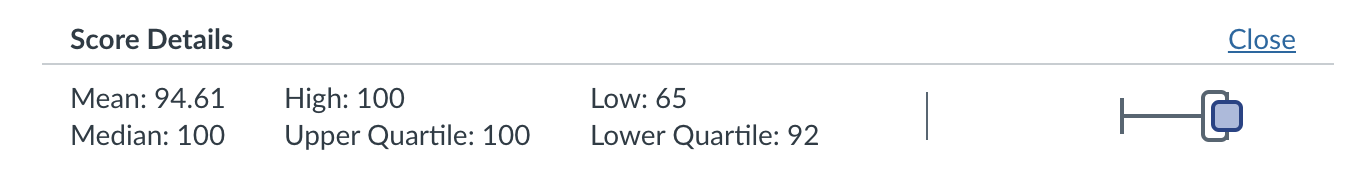
\includegraphics[width=1\linewidth]{image.png}
\end{figure}
\subsection{Problems}
Assume all functions are periodic with period 1, and let $a_n\left(\cdots\right)$ denote the Fourier coefficients of that function.
\begin{enumerate}
    \item Prove that, for $u, v \in V$ where $V$ is a real inner product space,
    \begin{align*}
        \langle u, v \rangle = \dfrac{1}{4} \left[ \norm{u+v}^2 - \norm{u-v}^2 \right]
    \end{align*}
    \item For continuous, periodic functions $f(x)$ and $g(x) := e^{6\pi ix} f(x)$, show that
    \begin{align*}
        a_n(g) = a_{n-3}(f)
    \end{align*}
    \item For continuous, periodic functions $f(x)$ and $g(x) := f(x+\frac{1}{2})$, show that
    \begin{align*}
        a_n(g) = (-1)^n \cdot a_n(f)
    \end{align*}
\end{enumerate}
\subsection{Solutions}
These solutions are transcribed from my original exam booklet, though were written up months after the course had already ended. A small amount of commentary was added because otherwise it would be too boring.
\subsubsection{Problem 1}
\begin{solution}
    We can prove this directly and quite easily:
    \begin{align}
        \dfrac{1}{4}\left( \norm{u + v}^2 - \norm{u - v}^2 \right) &= \dfrac{1}{4} \left[ \langle u+v,u+v \rangle - \langle u-v,u-v \rangle \right]
    \end{align}
    From here you could do this yourself, but we can just expand it if we don't want to expend any braincells for the other two problems which are supposedly harder.
    \begin{align}
        (13.1) &= \dfrac{1}{4} \left[ \langle u,u+v \rangle + \langle v,u+v \rangle - \langle u,u-v \rangle + \langle v,u-v \rangle \right]\\
        &= \dfrac{1}{4} \left[ \langle u,u \rangle + \langle u,v \rangle + \langle v,u \rangle + \langle v,v \rangle - \langle u,u \rangle + \langle u,v \rangle + \langle v,u \rangle - \langle v,v \rangle \right]\\
        &= \dfrac{1}{4} \left[ 2\langle u,v \rangle + 2\langle v,u \rangle \right]
    \end{align}
    Since $V$ is a real vector space,
    \begin{align}
        (13.4) = \dfrac{1}{4} \left[ 4 \langle u, v \rangle \right] = \langle u, v \rangle
    \end{align}
\end{solution}

\subsubsection{Problem 2}
\begin{solution}
    We can solve this by just writing it out and recalling how to do a substitution:
    \begin{align}
        a_n(g) &= \int_0^1 g(t) e^{-2\pi int} \dd{t}\\
        &= \int_0^1 e^{6\pi it} f(t) e^{-2\pi int} \dd{t}\\
        &= \int_0^1 f(t) e^{6\pi it -2\pi int} \dd{t}\\
        &= \int_0^1 f(t) e^{-2\pi i(n-3)t} \dd{t}\\
        &= \langle f(t), e^{2\pi i (n-3) t} \rangle\\
        &= a_{n-3}(f) \qedhere
    \end{align}
    Note that the conclusion from (13.9) to (13.10) follows from the fact that if we let
    \begin{align}
        a_m(f) = \langle f(t), e^{2\pi imt} \rangle
    \end{align}
    then set $m = n-3$ and the reasoning is trivial.
\end{solution}

\subsubsection{Problem 3}
\begin{solution}
    This is once again, a question that is solved by just writing it out:
    \begin{align}
        g(t) = f(t + 1/2) \implies a_n(g) &= \int_0^1 g(t) e^{-2\pi int} \dd{t}\\
        &= \int_0^1 f(t+1/2) e^{-2\pi int} \dd{t}
    \end{align}
    Use a substitution $u = t+1/2$ which gives $t = u-1/2$ and $\dd{t} = \dd{t}$. Then we get
    \begin{align}
        a_n(g) &= \int_{1/2}^{3/2} f(u) e^{-2\pi in(u - 1/2)} \dd{u}\\
        &= \int_{1/2}^{3/2} f(u) e^{-2\pi inu} e^{\pi in} \dd{u}\\
        &= \int_{1/2}^{3/2} (-1)^n f(u) e^{-2\pi inu} \dd{u}
    \end{align}
    Note that we leveraged the fact that $e^{\pi i n}$ equals $\pm 1$ depending on if $n$ is even or odd. After this there was some more annoying substitution, but the gist of the proof was that since $f(u)$ is periodic, we can phase shift the integral in (13.16) to be on $[0,1]$, and we get
    \begin{align}
        a_n(g) &= \int_0^1 (-1)^n  f(u) e^{2\pi in u} \dd{u}\\
        &= (-1)^n \int_0^1 f(u) e^{2\pi in u} \dd{u}\\
        &= (-1)^n a_n(f)
    \end{align}
\end{solution}
\subsection{Some notes}
I finished this in 20 minutes. It was too easy. Unfortunately for us at the time, we did not know that the final would be way harder.
    \section{Lecture 13}
\begin{enumerate}
    \item ``Complex numbers are intermediate steps.''
    \item ``It sounds crazy, but it works.''
\end{enumerate}
\subsection{Heat Equation}
We want some function
\begin{align}
    u(t, x): [0, \infty) \times \mathbb{L} \to \mathbb{R}
\end{align}
such that
\begin{align}
    \pdv{u}{t} &= \pdv[2]{u}{x}\\
    u(t_0, x) &= h(x)
\end{align}
Let $u(t,x)$ be a solution. Then, for every $t_0$, look at $x \to u(t_0, x)$ and Fourier expand:
\begin{align}
    u(t_0, x) = \sum U_n(t_0) \cdot e^{2\pi inx}
\end{align}
which implies
\begin{align}
    u(t, x) = \sum U_n(t) \cdot e^{2\pi inx}
\end{align}
Using this,
\begin{align}
    \pdv{u}{t} &= \sum U_n'(t) \cdot e^{2\pi inx}\\
    \pdv[2]{u}{x} &= \sum U_n(t) \cdot (-4\pi^2n^2) \cdot e^{2\pi inx}
\end{align}
which indicates
\begin{align}
    \sum U_n'(t) \cdot e^{2\pi inx} = \sum U_n(t) \cdot (-4\pi^2n^2) \cdot e^{2\pi inx}
\end{align}
Since $\{ e^{2\pi inx} \}$ is an orthonormal set, for two linear combinations to be equal, the coefficients must be equal, so 
\begin{align}
    U_n'(t) = U_n(t) \cdot (-4\pi^2n^2)
\end{align}
This is a simple ODE with solution
\begin{align}
    U_n(t) = c_n e^{(-4\pi^2n^2)t}
\end{align}
Plugging in $t=0$ to $u(0, x) = h(x)$,
\begin{align}
    h(x) = u(0, x) &= \sum_{n \in \mathbb{Z}} c_n e^{2\pi inx} & t = 0 \implies e^{\cdots} = 1
\end{align}
So, $c_n$ are the Fourier coefficients of $h(x)$, the boundary condition. Plugging in, this becomes a two step process:
\begin{enumerate}
    \item Fourier expand
    \begin{align}
        h(x) = \sum_{n \in \mathbb{Z}} c_n e^{2\pi in x}
    \end{align}
    \item Solution becomes
    \begin{align}
        u(t, x) &= \sum_{n \in \mathbb{Z}} c_n e^{(-4\pi^2n^2)t} e^{2\pi in x} & (13.5/10)
    \end{align}
\end{enumerate}
We now claim that $u(t, x)$ is real
\begin{lemma}
    If $h(x)$ is real, then $u(t, x)$ is real.
\end{lemma}
\begin{proof}
    \begin{align}
        h(x) \in \mathbb{R} &\implies c_n = \overline{c_{-n}}
    \end{align}
    If $\overline{U_n(t)} = U_{-n}(t)$, then $u(t, x)$ is also real. This is true:
    \begin{align}
        U_n(t) &= c_n \cdot e^{(-4\pi^2n^2)t}\\
        &= c_n \cdot e^{(-4\pi^2(-n)^2)t}
    \end{align}
    Taking the conjugate,
    \begin{align}
        \overline{U_n(t)} &= \overline{c_n \cdot e^{(-4\pi^2(-n)^2)t}}\\
        &= \overline{c_n} \cdot \overline{e^{(-4\pi^2(-n)^2)t}}\\
        &= c_{-n} \cdot {e^{(-4\pi^2(-n)^2)t}}\\
        &= U_{-n}(t)
    \end{align}
\end{proof}

\subsection{Wave Equation}
A similar process can be applied to the wave equation:
\begin{align}
    \pdv[2]{\Psi}{t} = \pdv[2]{\Psi}{x}
\end{align}
First, we claim
\begin{align}
    \Psi(t, x) = \sum_n U_n(t) \cdot e^{2\pi in x}
\end{align}
So,
\begin{align}
    \pdv[2]{\Psi}{t} &= \sum_n U_n''(t) \cdot e^{2\pi in x}\\
    \pdv[2]{\Psi}{x} &= \sum_n U_n(t) \cdot (-4\pi^2n^2) \cdot e^{2\pi in x}
\end{align}
So,
\begin{align}
    \sum_n U_n''(t) \cdot e^{2\pi in x} = \sum_n U_n(t) \cdot (-4\pi^2n^2) \cdot e^{2\pi in x}
\end{align}
and by the same linear independence argument as applied in (13.9),
\begin{align}
    U_n''(t) = U_n(t) \cdot (-4\pi^2n^2)
\end{align}
which is another simple ODE, with solution
\begin{align}
    U_n(t) = a_n e^{2\pi in t} + b_n e^{-2\pi in t}
\end{align}
So, the general solution to the wave equation has form
\begin{align}
    \Psi(t, x) &= \sum_n \left[ a_n e^{2\pi in t} + b_n e^{-2\pi in t} \right] e^{2\pi inx}\\
    &= \sum_n a_n e^{2\pi in (x + t)} + \sum_n b_n e^{2\pi in (x - t)}
\end{align}
which indicates the solution is the sum of two functions moving in opposite directions at some velocity.
    \section{Lecture 14}
\subsection{More on the Heat Equation / Diffusion Equation}
The equation
\begin{align}
    \pdv{u}{t} = \kappa \pdv[2]{u}{x}
\end{align}
Suppose we want to solve this on the interval
\begin{align}
    [0, L]
\end{align}
as opposed to
\begin{align}
    [0, 1]
\end{align}
Generally, on $[0, 1]$, the set of functions
\begin{align}
    \{ e^{2\pi in x} \}
\end{align}
is used as an orthonormal basis. On $[0, L]$ we instead use
\begin{align}
    \{ e^{\frac{2\pi in x}{L}} \}
\end{align}
as the orthogonal basis.
\begin{proof}[Solution]
    Expand $u(t, x)$ using the new basis in (14.5), i.e.
    \begin{align}
        u(t, x) = \sum U_n(t) \cdot e^{\frac{2\pi in x}{L}}
    \end{align}
    Now,
    \begin{align}
        \pdv{u}{t} &= \sum U_n'(t) \cdot e^{\frac{2\pi in x}{L}}\\
        &= \kappa \pdv[2]{u}{x}\\
        &= \sum U_n(t) \cdot \kappa\left( \frac{-4\pi^2 n^2}{L^2} \right) \cdot e^{\frac{2\pi in x}{L}}
    \end{align}
    So,
    \begin{align}
        U_n'(t) &= U_n(t) \cdot \kappa\left( \frac{-4\pi^2 n^2}{L^2} \right)\\
        &= \frac{-4\pi^2 n^2 \kappa}{L^2} U_n(t)
    \end{align}
    The solution to this is
    \begin{align}
        c_n e^{\frac{-4\pi^2n^2\kappa}{L^2}t} \cdot e^{\frac{2\pi in x}{L}}
    \end{align}
    So, the general solution becomes
    \begin{align}
        \boxed{\sum_n c_n e^{\dfrac{-4\pi^2n^2\kappa}{L^2}t} \cdot e^{\dfrac{2\pi in x}{L}}}
    \end{align}
    To find $c_n$, do
    \begin{align}
        \left\langle u(0, x), e^{\frac{2\pi in x}{L}} \right\rangle &= \int_0^L \left[ h(x) \cdot e^{\frac{2\pi in x}{L}} \right] \dd{x}\\
        &= \left\langle \sum_k c_k e^{\frac{2\pi ik x}{L}}, e^{\frac{2\pi in x}{L}} \right\rangle\\
        &= c_n \int_0^L 1 \dd{x} & \text{all vanish except $k = n$}\\
        &= c_nL
    \end{align}
    so
    \begin{align}
        \boxed{c_nL = \int_0^L \left[ h(x) \cdot e^{\frac{2\pi in x}{L}} \right] \dd{x}}
    \end{align}
    \begin{lemma}
        \begin{align}
            \lim_{t \to \infty} u(t, x) &= c_n\\
            &= \frac{1}{L} \int_0^L h(x) \dd{x}
        \end{align}
        i.e. as time goes to infinity, the temperature of all points on some one-dimensional rod converge to the average temperature of the rod.
        \begin{proof}
            Pretty easy based on the above equations. Take $t \to \infty$ in (14.13).
        \end{proof}
    \end{lemma}
\end{proof}

\subsection{Continuity}
\begin{proposition}
    If $f: [0, 1] \to \mathbb{C}$ is continuous, then
    \begin{enumerate}
        \item The Fourier coefficients tend to zero
        \begin{align}
            a_n(f) \to 0
        \end{align}
    \end{enumerate}
\end{proposition}
\begin{proof}
    Implied by Lemma 9.5
\end{proof}
\begin{proposition}
    If
    \begin{align}
        \sum \abs{a_n} < \infty && \text{absolutely converges}
    \end{align}
    then the series
    \begin{align}
        \abs{a_n \cdot e^{2\pi in x}}
    \end{align}
    converges to a continuous function.
\end{proposition}
\begin{proof}
    \begin{enumerate}
        \item The sum in (14.23) absolutely converges
        \begin{align}
            \sum \abs{a_n \cdot e^{2\pi in x}} = \sum \abs{a_n} <  \infty
        \end{align}
        (note the cancellation because $\abs{e^{2\pi in x}} = 1$) so thus also converges.
        \item Let $f(x) = \sum a_n e^{2\pi in x}$. We claim that
        \begin{align}
            \sum a_n e^{2\pi in x} \to f(x)
        \end{align}
        uniformly.
        \begin{proof}
            Let $\varepsilon > 0$ be given. Since
            \begin{align}
                \sum \abs{a_n} < \infty
            \end{align}
            there is some $N$ such that
            \begin{align}
                \sum_{\abs{n} > N} \abs{a_n} < \varepsilon
            \end{align}
            So, for every $x$,
            \begin{align}
                \abs{f(x) - \sum_{n = -N}^N a_n e^{2\pi in x}} < \varepsilon
            \end{align}
            Removing these elements yields
            \begin{align}
                \abs{\sum_{\abs{n}>N} a_n e^{2\pi in x}} &\le \abs{\sum_{\abs{n}>N} a_n e^{2\pi in x}}\\
                &\le \sum_{\abs{n}>N} \abs{a_n} \cdot \abs{{e^{2\pi in x}}}\\
                &\le \sum_{\abs{n}>N} \abs{a_n}\\
                &\le \varepsilon
            \end{align}
        \end{proof}
        \item We now claim $f(x)$ is continuous, so we need to show that $\forall x_0 \in [0, 1]$, and $\varepsilon > 0$ if $h$ is small enough,
        \begin{align}
            \abs{f(x_0 + h) - f(x_0)} < \varepsilon
        \end{align}
        \begin{proof}
            \begin{align}
                \abs{f(x_0 + h) - f(x_0)} &= \abs{\sum a_n \left[ e^{2\pi in (x_0 + h)} - e^{2\pi in x_0} \right]}\\
                &= \abs{\sum a_n e^{2\pi in x_0} \left[ e^{2\pi in h} - 1 \right]}\\
                &\le \sum \abs{a_n e^{2\pi in x_0}} \cdot \abs{ e^{2\pi in h} - 1}
            \end{align}
            This equals
            \begin{align}
                (14.36) &= \sum_{\abs{n} \le N} \abs{a_n e^{2\pi in x_0}} \abs{ e^{2\pi in h} - 1} + \sum_{\abs{n} > N} \abs{a_n e^{2\pi in x_0}} \abs{ e^{2\pi in h} - 1}\\
                &\le \sum_{\abs{n} \le N} \abs{a_n e^{2\pi in x_0}} \abs{ e^{2\pi in h} - 1} + 2\sum_{\abs{n} > N} \abs{a_n}
            \end{align}
            Claim: the inequality
            \begin{align}
                (14.38) \le 14MN^2\abs{h} + 2\varepsilon
            \end{align}
            is true.
            \begin{proof}[Reasoning]
                After plugging in (14.32), we simply need to show
                \begin{align}
                    \sum_{\abs{n} \le N} \abs{a_n e^{2\pi in x_0}} \abs{ e^{2\pi in h} - 1} \le 14MN^2\abs{h}
                \end{align}
                To do this,
                \begin{align}
                    \abs{a_n e^{2\pi in x_0}} &\le \abs{a_n}\\
                    &\le M & \text{Upper bound; $\abs{a_n}$ is abs. cvngt.}
                \end{align}
                and
                \begin{align}
                    \abs{ e^{2\pi in h} - 1} &\le 2\pi n \abs{h}\\
                    &\le 7 N \abs{h}
                \end{align}
                because $\abs{h}$ is small, i.e this difference is smaller than the corresponding arc length, given the angle is very small. So, summing $2N$ of these elements,\footnote{$a_0$ would be the $(2N+1)$-th element, but at $n = 0$, $e^{2\pi in h} - 1 = 0$}
                \begin{align}
                    \sum_{\abs{n} \le N} \abs{a_n e^{2\pi in x_0}} \cdot \abs{ e^{2\pi in h} - 1} \le 14MN^2\abs{h}
                \end{align}
            \end{proof}
            So, based on this, if
            \begin{align}
                \abs{h} < \dfrac{\varepsilon}{14MN^2}
            \end{align}
            then
            \begin{align}
                \abs{f(x_0 + h) - f(x_0)} < \varepsilon + 2\varepsilon = 3\varepsilon
            \end{align}
            So, use $\varepsilon = \varepsilon/3$, and the proof is complete.
        \end{proof}
    \end{enumerate}
\end{proof}
    \section{Lecture 15}
\subsection{More on Continuity}
\begin{lemma}
    $f: \mathbb{L} \to \mathbb{C}$ is continuously differentiable $\implies$ $n \cdot a_n(f) \to 0$
\end{lemma}
\begin{proof}
    Recall
    \begin{align}
        a_n(f') = -2\pi in \cdot a_n(f)
    \end{align}
    Since $f$ is continuously differentiable, $f'$ is continuous, so
    \begin{align}
        a_n(f') \to 0
    \end{align}
\end{proof}
In the other direction\footnote{In class, this was actually written mirrored on the board.}
\begin{lemma}
    \begin{align}
        \begin{cases}
            \sum_{n \in \mathbb{Z}} \underbrace{\abs{n a_n(f)}}_{b_n} < \infty\\
            f\text{ continuous}
        \end{cases} \implies f \text{ is continously differentiable}
    \end{align}
\end{lemma}
\begin{proof}
    From Lecture 14 (implied?)
    \begin{align}
        \sum -2\pi in \cdot a_n(f) \cdot e^{2\pi in x} < \infty
    \end{align}
    converges (pointwise and uniformly) to a continuous function $g$. Then, let
    \begin{align}
        h(x) = \int g(x) \dd{x}
    \end{align}
    Then,
    \begin{align}
        h'(x) = g(x)
    \end{align}
    so,
    \begin{align}
        a_n(g) = -2\pi in \cdot a_n(h) &\implies a_n(h) = \frac{a_n(g)}{-2\pi in} = \frac{-2\pi in \cdot a_n(f)}{-2\pi in}\\
        &\implies a_n(h) = a_n(f)
    \end{align}
    i.e. the Fourier coefficients are the same.
\end{proof}
\begin{lemma}
    It remains that we need to prove that for functions $h, f \in \mathcal{F}$
    \begin{align}
        a_n(h) = a_n(f) \implies h = f
    \end{align}
\end{lemma}
\begin{proof}
    \begin{align}
        \norm{h-f}^2 &= \int_0^1 \left(h(x) - f(x)\right)^2 \dd{x}\\
        &= \sum_n \abs{a_n(h-f)}^2
    \end{align}
    But,
    \begin{align}
        (15.11) = \sum_n \abs{a_n(h)-a_n(f)}^2 = 0
    \end{align}
    Furthermore, if for any $x_0$,
    \begin{align}
        h(x_0) \ne f(x_0)
    \end{align}
    then we would get
    \begin{align}
        h(x) \ne f(x)
    \end{align}
    over some interval $I \subset [0,1]$, but then
    \begin{align}
        &\int_I \abs{h(x) - f(x)}^2 \dd{x} > 0\\
        &\implies \int_0^1 \abs{h(x) - f(x)}^2 \dd{x} \ge \int_I \abs{h(x) - f(x)}^2 \dd{x} > 0
    \end{align}
    This contradicts (15.12), so for all $x_0$,
    \begin{align}
        h(x_0) = f(x_0)
    \end{align}
    which implies
    \begin{align}
        h - f = 0
    \end{align}
\end{proof}
\subsection{Summary}
\begin{lemma}
    If $f$ is $k$-ce continuously differentiable, then $n^k \cdot a_n(f) \to 0$
\end{lemma}
\begin{lemma}
    If
    \begin{align}
        \sum \abs{a_n(f) \cdot n^k} \to 0
    \end{align}
    then $f$ is $k$-ce continuously differentiable.
\end{lemma}
\subsection{A Corollary}
\begin{lemma}
    $f$ is $\infty$-ce differentiable $\iff$ for every $k$, $n^k \cdot a_n(f) \to 0$
\end{lemma}
\noindent Now it's an if and only if, so let's prove it.
\begin{proof}
    We saw $\Rightarrow$ in Lemmas 16.1-3. What about $\Leftarrow$? Assume the right hand side. Then, we want to show that
    \begin{align}
        f \text{ is $p$ times differentiable}
    \end{align}
    Then, for $k = p + 2$,
    \begin{align}
        n^{p+2} \cdot a_n(f) \to 0
    \end{align}
    and
    \begin{align}
        \abs{n^{p+2} \cdot a_n(f)} < M
    \end{align}
    for some $M$. But,
    \begin{align}
        \sum \abs{n^p \cdot a_n(f)} &= \sum \abs{n^{p+2} \cdot a_n(f)} \frac{1}{n^2}\\
        &\le \sum M \frac{1}{n^2} < \infty
    \end{align}
    And by Lemma 16.5 this proves that $f$ has $p$ derivatives. This can be applied for all $p \in \mathbb{Z}$, and if we replace all instances of $p$ with $k$, this proves the Lemma.\footnote{This proof is bad induction.}
\end{proof}

\subsection{Heat Equation Again}
Let $h(x)$ be a continuous function and let $u(t, x)$ be a solution of the heat equation with initial condition $u(0, x) = h(x)$. This solution is
\begin{align}
    u(t, x) = \sum c_n \cdot e^{-4\pi^2n^2t} \cdot e^{2\pi in x}
\end{align}
Because $h(x)$ is continuous, $c_n \to 0$ and are bounded by some constant $\max_{x\in[0,1]}\:h(x)$. So,
\begin{align}
    u(0.000001, x) = \sum c_n \cdot e^{-4\pi^2n^2(0.000001)} \cdot e^{2\pi in x}
\end{align}
This decays faster than any polynomial\footnote{This was not proven}. So by Lemma 26, this implies
\begin{align}
    u(0.000001, x) \text{ is $\infty$-ce differentiable}
\end{align}

\subsection{Alcoholism and Convolutions}
Let
\begin{align}
    g(t):= \text{ BAC $t$ minutes after taking a shot}
\end{align}
Suppose you drink $a_0$ shots at $t=0$, $a_1$ shots at $t=1$, $\cdots$, $a_n$ shots at $t=n$. In general, the total BAC at time $t$ is
\begin{align}
    a_0\cdot g(t) + a_1\cdot g(t-1) + \cdots
\end{align}
These are such important questions that they lead to two definitions
\begin{definition}
    The convolution of two sequences $a_n$ and $b_n$ ($n \in \mathbb{Z}$) is the sequence
    \begin{align}
        (a * b)_n := \sum_{k \in \mathbb{Z}} a_k b_{n-k}
    \end{align}
\end{definition}
\noindent And, for periodic functions,
\begin{definition}
    The convolution of two periodic functions $f$ and $g$ is
    \begin{align}
        (f * g)(x) := \int_0^1 f(t)\cdot g(x-t) \dd{t}
    \end{align}
\end{definition}
\noindent We claim
\begin{theorem}
    \begin{align}
        a_n(f * g) = a_n(f) \cdot a_n(g)
    \end{align}
\end{theorem}
\begin{proof}
    \begin{align}
        a_n(f * g) &= \int_0^1 (f*g)(x) e^{-2\pi in x}\\
        &= \int_0^1 \int_0^1 f(t) \cdot g(x-t) \cdot e^{-2\pi in t} \cdot e^{-2\pi in (x-t)} \dd{t} \dd{x}\\
        &= \int_0^1 \int_0^1 f(t) \cdot g(x-t) \cdot e^{-2\pi in t} \cdot e^{-2\pi in (x-t)} \dd{x} \dd{t}\\
        &= \int_0^1 f(t) \cdot e^{-2\pi in t} \cdot \int_0^1 g(x-t)  \cdot e^{-2\pi in (x-t)} \dd{x} \dd{t}
    \end{align}
    Fix $y = x-t$,
    \begin{align}
        a_n(f * g) &= \int_0^1 f(t) \cdot \cdot e^{-2\pi in t} \dd{t} \cdot \int_{-t}^{1-t} g(y)  \cdot e^{-2\pi in y} \dd{y} \\
        &= \int_0^1 f(t) \cdot e^{-2\pi in t} \dd{t} \cdot \int_{0}^{1} g(y) \cdot e^{-2\pi in y} \dd{y}\\
        &= a_n(f) \cdot a_n(g)
    \end{align}
\end{proof}
    \section{Lecture 16}
``It's convoluted''
\subsection{Redefining Convolution}
Recall that for periodic functions
\begin{definition}
    The convolution of \textbf{two periodic functions} $f$ and $g$ is
    \begin{align}
        (f * g)(x) := \int_0^1 f(t)\cdot g(x-t) \dd{t}
    \end{align}
\end{definition}
It is quite trivial to prove
\begin{lemma}
    \begin{align}
        a_n(f * g) = a_n(g * f)
    \end{align}
    and
    \begin{align}
        f*g = g*f
    \end{align}
\end{lemma}
via simple commutativity. Note that (16.1) does not apply to non-periodic functions, which would be some integral from $-\infty$ to $+\infty$.
\begin{lemma}
    $$f*g = g*f$$
    but in a different way.
\end{lemma}
\begin{proof}
    \begin{align}
        \int_0^1 f(t)\cdot g(x-t) \dd{t} &= -\int_x^{x-1} f(x-s)\cdot g(s) \dd{s}\\
        &= \int_0^1 f(x-s)\cdot g(s) \dd{s} & \text{It's periodic}
    \end{align}
\end{proof}
\noindent Blurring is an example of a convolution.
\begin{align}
    (B_\varepsilon f)(x) = \frac{1}{\varepsilon} \int_0^\varepsilon f(x - s) \dd{s}
\end{align}
We can define
\begin{align}
    1_{[0,\varepsilon]}(x) := \begin{cases}
        1 & x \in [0, \varepsilon]\\
        0 & \text{else}
    \end{cases}
\end{align}
And it can be shown that
\begin{align}
    (B_\varepsilon f)(x) = \left(f * \left[ \frac{1}{\varepsilon} 1_{[0,\varepsilon]} \right]\right)
\end{align}

\subsection{A Black Box}
Suppose there is a signal
\begin{align}
    f: \mathbb{R} \to \mathbb{C}
\end{align}
a system
\begin{align}
    T
\end{align}
and a response
\begin{align}
    Tf: \mathbb{R} \to \mathbb{C}
\end{align}
from the signal.
\subsection{Time Variance}
Suppose there is some system
\begin{align}
    S_a
\end{align}
that time shifts an input function
\begin{align}
    f(x)
\end{align}
into
\begin{align}
    f(x + a)
\end{align}
\begin{definition}
    A system $T$ is called
    \begin{enumerate}
        \item \textbf{Time Invariant} if $TS_a = S_aT$.
        \item \textbf{Linear} if $T(\lambda f+g) = \lambda T(f) + T(g)$, which holds true in approximations, but is generally not true.
    \end{enumerate}
\end{definition}
\subsection{The Fundamental Theorem of Engineering}
\begin{theorem}
    \textbf{(The Fundamental Theorem of Engineering)} Suppose $T$ is linear and time-invariant. Then,
    \begin{enumerate}
        \item $T \left( e^{2\pi in t} \right)$ is always a multiple of $e^{2\pi in t}$, i.e.
        \begin{align}
            e^{2\pi in t}
        \end{align}
        are the eigenvalues of $T$.
        \item If
        \begin{align}
            \sum_{n \in \mathbb{Z}} \abs{\lambda_n} < \infty
        \end{align}
        then there exists a function $g$ such that
        \begin{align}
            Tf = f * g
        \end{align}
        i.e. all linear, time-invariant systems are just convolutions.
    \end{enumerate}
\end{theorem}
\subsection{The Proof}
First, the eigenvalues.
\begin{proof}
    Denote $f_n = T e^{2\pi in t}$. Then,
    \begin{align}
        S_a T e^{2\pi in t} = T S_a e^{2\pi in t}
    \end{align}
    which becomes
    \begin{align}
        S_a f_n &= T\left[ e^{2\pi in (t+a)} \right]\\
        &= T\left[ e^{2\pi in t} \cdot e^{2\pi in a} \right]\\
        &= e^{2\pi in a} \cdot T\left[ e^{2\pi in t} \right]\\
        &= e^{2\pi in a} \cdot f_n
    \end{align}
    At $t=0$,
    \begin{align}
        f_n(0 + a) &= (S_a f_n)(0)\\
        &= e^{2\pi in a} \cdot f_n(0)
    \end{align}
    Hence, let\footnote{Some variable is wrong here.} $f_n(0) := \lambda_n$
    \begin{align}
        f_n(a) = \lambda_n \cdot e^{2\pi in a} \implies f_n = \lambda_n \cdot e^{2\pi in t}
    \end{align}
    so
    \begin{align}
        T(e^{2\pi in t}) = \lambda_n \cdot e^{2\pi in t}
    \end{align}
    proving that the result of applying the linear transformation is a multiple of that function.
\end{proof}
\noindent Next, that $T$ is a convolution.
\begin{proof}
    Let $g(t) = \sum \lambda_n \cdot e^{2\pi in t}$. We claim
    \begin{align}
        Tf = f*g \mid \forall f
    \end{align}
    By definition, $g(t)$ is continuous. If we can show
    \begin{align}
        a_n(Tf) = a_n(f * g)
    \end{align}
    then we will have proven that the two are the same.
    \begin{align}
        f(t) &= \sum a_n(f) \cdot e^{2\pi in t}\\
        Tf &= T\left[ \sum a_n(f) \cdot e^{2\pi in t} \right]\\
        &= \sum a_n(f) \cdot T(e^{2\pi in t}) & \text{linearity}\\
        &= \sum a_n(f) \cdot \lambda_n \cdot e^{2\pi in t} & \text{Part 1 of Theorem 17.5}
    \end{align}
    So,
    \begin{align}
        a_n(Tf) = a_n(f) \cdot \lambda_n
    \end{align}
    but $\lambda_n$ are just the Fourier coefficients of $g(t)$ by definition, so
    \begin{align}
        a_n(Tf) = a_n(f) \cdot a_n(g) = a_n(f*g) && \text{PSet 4 Problem 2}
    \end{align}
    So,
    \begin{align}
        Tf = f * g && \text{Fourier coefficients equal}
    \end{align}
\end{proof}
    \section{Lecture 17}
``One of our main tools to show convergence is to strength it and show absolute convergence.''
\subsection{The Fourier Transform}
\begin{definition}
    Let $f: \mathbb{R}\to\mathbb{C}$. The, the Fourier Transform of $f$ is given by
    \begin{align}
        \hat{f}(\xi) = \dfrac{1}{\sqrt{2\pi}} \int_{-\infty}^\infty f(x) \cdot e^{-ix\xi} \dd{x}
    \end{align}
\end{definition}
\begin{definition}
    Let $V$ be the collection of functions
    \begin{align}
        f: \mathbb{R}\to\mathbb{C}
    \end{align}
    that satisfy
    \begin{enumerate}
        \item There is $M$ such that $\abs{f(x)} \le M$
        \item $f$ is piecewise differentiable
        \item $\int_{-\infty}^\infty \abs{f(x)} \dd{x} < \infty$
    \end{enumerate}
\end{definition}

\subsection{Several Lemmas}
\begin{lemma}
    $V$ is a vector space.
\end{lemma}
\begin{proof}
    The first two are trivial\footnote{Nir's words not mine}. The only non obvious claim is that if
    \begin{align}
        \int_{-\infty}^\infty \abs{f(x)} \dd{x} < \infty \qand \int_{-\infty}^\infty \abs{g(x)} \dd{x} < \infty
    \end{align}
    then
    \begin{align}
        \int_{-\infty}^\infty \abs{f(x) + g(x)} \dd{x} < \infty
    \end{align}
    By the Triangle Inequality,
    \begin{align}
        \int_{-\infty}^\infty \abs{f(x) + g(x)} \dd{x} &\le \int_{-\infty}^\infty \abs{f(x)} + \abs{g(x)} \dd{x}\\
        &\le \int_{-\infty}^\infty \abs{f(x)} \dd{x} + \int_{-\infty}^\infty \abs{g(x)} \dd{x}
    \end{align}
    Both of these are bounded, so
    \begin{align}
        \int_{-\infty}^\infty \abs{f(x) + g(x)} \dd{x} < \infty
    \end{align}
\end{proof}
\begin{lemma}
    If $f, g \in V$, then
    \begin{enumerate}
        \item $\int_{-\infty}^\infty \abs{f(x)}^2 \dd{x} < \infty$
        \item $\int_{-\infty}^\infty f(x)\cdot g(x) \dd{x} < \infty$
    \end{enumerate}
\end{lemma}
\begin{proof}
    First, to show
    \begin{align}
        \int_{-\infty}^\infty \abs{f(x)}^2 \dd{x} < \infty
    \end{align}
    let $f \in V$, then
    \begin{align}
        \abs{f(x)} \le M
    \end{align}
    Then,
    \begin{align}
        \int_{-\infty}^\infty \abs{f(x)}^2 \dd{x} &\le \int_{-\infty}^\infty M \cdot \abs{f(x)} \dd{x}\\
        &\le M\cdot\int_{-\infty}^\infty \abs{f(x)} \dd{x}\\
        &\le \infty & \int_{-\infty}^\infty \abs{f(x)} \dd{x} < \infty
    \end{align}
    Second, to show
    \begin{align}
        \int_{-\infty}^\infty f(x)\cdot g(x) \dd{x} < \infty
    \end{align}
    we can show that
    \begin{align}
        \int_{-\infty}^\infty \abs{f(x)\cdot g(x)} \dd{x} < \infty
    \end{align}
    i.e. show absolute convergence. Then,
    \begin{align}
        \int_{-\infty}^\infty \abs{f(x)\cdot g(x)} \dd{x} &\le \int_{-\infty}^\infty \abs{f(x)} \cdot \abs{g(x)} \dd{x}\\
        &\le M \cdot \int_{-\infty}^\infty \abs{g(x)} \dd{x} < \infty
    \end{align}
\end{proof}
\begin{definition}
    The inner product on $V$ is
    \begin{align}
        \langle f, g \rangle = \int_{-\infty}^\infty f(x) \cdot \overline{g(x)} \dd{x}
    \end{align}
    and converges because of Lemma 18.4.
\end{definition}

\subsection{Some Analogue Proofs}
\begin{lemma}
    If $f \in V$, then $\hat{f}$ exists and $\hat{f}$ is continuous.
\end{lemma}
\begin{proof}
    We \textbf{first want to show $\hat{f}$ exists}, so we can show it is finite
    \begin{align}
        \int_{-\infty}^\infty f(x) \cdot e^{-ix\xi} \dd{x} < \infty
    \end{align}
    We can show absolute convergence
    \begin{align}
        \int_{-\infty}^\infty \abs{f(x) \cdot e^{-ix\xi}} \dd{x} < \infty
    \end{align}
    Indeed,
    \begin{align}
        \int_{-\infty}^\infty \abs{f(x) \cdot e^{-ix\xi}} \dd{x} &\le \int_{-\infty}^\infty \abs{f(x)} \cdot \abs{e^{-ix\xi}} \dd{x}\\
        &= \int_{-\infty}^\infty \abs{f(x)} \dd{x} < \infty
    \end{align}
    by $f \in V$, so (17.18) absolutely converges and thus also converges. \textbf{Next, to show continuity}, we want to show
    \begin{align}
        \lim_{\xi \to \eta} \hat{f}(\xi) = \hat{f}(\eta)
    \end{align}
    or
    \begin{align}
        \lim_{\xi \to \eta} \dfrac{1}{\sqrt{2\pi}} \int_{-\infty}^\infty f(x) \cdot e^{ix\xi} \dd{x} = \dfrac{1}{\sqrt{2\pi}} \int_{-\infty}^\infty f(x) \cdot e^{ix\eta} \dd{x}
    \end{align}
    We can prove this using $\varepsilon-\delta$; or, if $\abs{\xi - \eta}$ is very small, then
    \begin{align}
        \abs{\dfrac{1}{\sqrt{2\pi}} \int_{-\infty}^\infty f(x) \cdot \left[e^{ix\xi} - e^{ix\eta}\right] \dd{x}} < \varepsilon
    \end{align}
    \begin{proof}
        Fix $\varepsilon$. Then, by assumption,
        \begin{align}
            \int_{-\infty}^\infty \abs{f(x)} \dd{x} < \infty
        \end{align}
        This means that there is some $T$ such that
        \begin{align}
            \int_{-\infty}^\infty \abs{f(x)} \dd{x} \approx \int_{-T}^T \abs{f(x)} \dd{x}
        \end{align}
        which would imply
        \begin{align}
            \left[\int_{-\infty}^{-T} \abs{f(x)} \dd{x} \qand \int_{T}^\infty \abs{f(x)} \dd{x}\right] < \varepsilon
        \end{align}
        Next,
        \begin{align}
            \abs{\hat{f}(\xi) - \hat{f}(\eta)} = \abs{\int_{-\infty}^\infty f(x) \left[ e^{ix\xi} - e^{ix\eta} \right] \dd{x}}
        \end{align}
        Now comes the trick of the proof. We rewrite the integral in (17.28) as
        \begin{align}
            \int_{-\infty}^{-T} \cdots + \int_{-T}^{T} \cdots + \int_{T}^{\infty} \cdots
        \end{align}
        Define $\zeta := \left[ e^{ix\xi} - e^{ix\eta} \right]$. Then, using the Triangle Inequality,
        \begin{align}
            (17.28) &\le \int_{-\infty}^{-T} \abs{f(x)} \cdot \abs{\zeta} \dd{x} + \int_{-T}^{T} \abs{f(x)} \cdot \abs{\zeta} \dd{x} + \int_{T}^{\infty} \abs{f(x)} \cdot \abs{\zeta} \dd{x}
        \end{align}
        But, $\abs{\zeta} \le 2$. So,
        \begin{align}
            (17.28) &\le 2\int_{-\infty}^{-T} \abs{f(x)} \dd{x} + \int_{-T}^{T} \abs{f(x)} \cdot \abs{\zeta} \dd{x} + 2\int_{T}^{\infty} \abs{f(x)} \dd{x}
        \end{align}
        Using (17.27),
        \begin{align}
            (17.28) &\le 4\varepsilon + \int_{-T}^{T} \abs{f(x)} \cdot \abs{\zeta} \dd{x}\\
            &\le 4\varepsilon + \int_{-T}^{T} \abs{f(x)} \cdot \abs{e^{ix\xi} - e^{ix\eta}} \dd{x}\\
            &\le 4\varepsilon + \int_{-T}^{T} M \cdot \abs{x} \cdot \abs{\xi - \eta} \dd{x}\\
            &\le 4\varepsilon + 2TM \cdot T \cdot \abs{\xi - \eta}\\
            &\le 4\varepsilon + 2T^2M \cdot \abs{\xi - \eta}
        \end{align}
        So
        \begin{align}
            \abs{\xi - \eta} < \frac{\varepsilon}{2T^2M} \implies \abs{\hat{f}(\xi) - \hat{f}(\eta)} < 5\varepsilon
        \end{align}
        so if $\varepsilon = \frac{\varepsilon}{5}$, then
        \begin{align}
            \abs{\hat{f}(\xi) - \hat{f}(\eta)} < \varepsilon
        \end{align}
    \end{proof}
\end{proof}

    \section{Lecture 18}
``I again don't remember so I'll guess.''

\subsection{The Fourier Transform Revisited}
Recall
\begin{definition}
    Let $f: \mathbb{R}\to\mathbb{C}$. The, the Fourier Transform of $f$ is given by
    \begin{align}
        \hat{f}(\xi) = \dfrac{1}{\sqrt{2\pi}} \int_{-\infty}^\infty f(x) \cdot e^{-ix\xi} \dd{x}
    \end{align}
\end{definition}

\subsection{Some (more) Properties}
``In all of these examples, I forgot to divide by $1/\sqrt{2\pi}$, but it doesn't matter.''
\begin{enumerate}
    \item Linearity.
    \begin{align}
        \widehat{\left[f + g\right]} = \widehat{f} + \widehat{g}
    \end{align}
    \begin{proof}
        It's quite trivial to prove this using (18.1).
    \end{proof}
    \item Dilation. If $g(x) = f(ax)$, then
    \begin{align}
        \hat{g}(\xi) = \dfrac{1}{a} \hat{f}(\xi/a)
    \end{align}
    \begin{proof}
        Doing a substitution $y = ax$ and $\dd{y} = a\dd{x}$,
        \begin{align}
            \hat{g}(\xi) = \int f(ax) e^{-ix \xi} \dd{x} = \frac{1}{a}\int f(y) e^{-iy \frac{\xi}{a}} \dd{y}
        \end{align}
    \end{proof}
    \item Translation. If $g(x) = f(x+a)$, then $\hat{g}(\xi) = e^{ia\xi} \hat{f}(\xi)$, i.e. the Fourier transformation is multiplied by some trigonometric wave.
    \begin{proof}
        \begin{align}
            \hat{g}(\xi) = \int f(x+a) e^{-ix \xi} \dd{x}
        \end{align}
        Using $y = x + a$,
        \begin{align}
            \hat{g}(\xi) &= \int f(y) e^{-i(y-a) \xi} \dd{y}\\
            &= e^{ia\xi} \int f(y) e^{-iy \xi} \dd{y}
        \end{align}
        which equals
        \begin{align}
            \hat{g}(\xi) = e^{ia\xi} \hat{f}(\xi)
        \end{align}
    \end{proof}
    \item Modulation. If $g(x) = f(x) \cdot e^{iax}$, then
    \begin{align}
        \hat{g}(\xi) = \hat{f}(\xi - a)
    \end{align}
    \begin{proof}
        \begin{align}
            \hat{g}(\xi) &= \int f(x) \cdot e^{iax} \cdot e^{-ix\xi} \dd{x}\\
            &= \int f(x) \cdot e^{-ix(\xi-a)} \dd{x}\\
            &= \hat{f}(\xi - a)
        \end{align}        
    \end{proof}
\end{enumerate}

\subsection{Radio}
\subsubsection{AM (Amplitude Modulation) Radio}
Let $S(x)$ be some signal. AM radio broadcasts $S(x) \cdot e^{ixa}$, or the signal modulated by some trignometric wave. Some circuit then takes the Fourier transform of a signal, throws away all frequencies that don't matter, and then does an inverse Fourier transform. So, all other stations become damped.
\begin{align}
    \widehat{S(\xi) \cdot e^{i\xi a}} = \hat{S}(\xi + a)
\end{align}

\subsubsection{FM (Frequency Modulation) Radio}
Amplitude is held constant, but frequency changes.
\begin{figure}[h!]
    \centering
    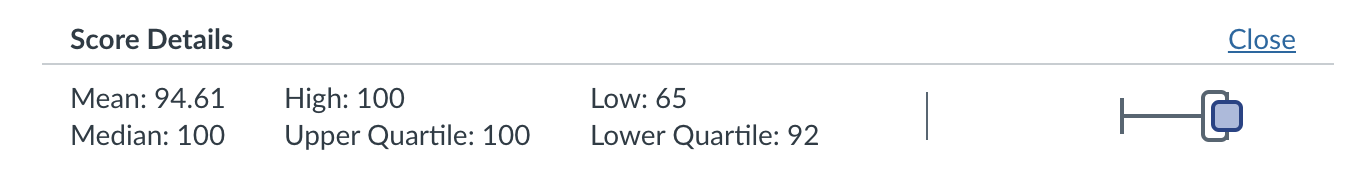
\includegraphics[width=0.3\linewidth]{image.png}
    \caption{Frequency modulation}
\end{figure}

\subsection{Convolutions for Nonperiodic Functions}
\begin{definition}
    If $f, g \in V$, then their convolution is
    \begin{align}
        (f * g)(x) = \int_{-\infty}^\infty f(t) \cdot g(x-t) \dd{t}
    \end{align}
\end{definition}
\begin{enumerate}
    \setcounter{enumi}{4}
    \item Convolutions.
    \begin{align}
        \boxed{\widehat{f*g}(\xi) = \sqrt{2\pi} \cdot \hat{f}(\xi) \cdot \hat{g}(\xi)}
    \end{align}
    \begin{proof}
        \begin{align}
            \widehat{f*g}(\xi) &= \dfrac{1}{\sqrt{2\pi}} \int (f*g)(x) e^{-ix\xi} \dd{x}\\
            &= \dfrac{1}{\sqrt{2\pi}} \int \left[ \int f(t) \cdot g(x-t) \dd{t} \right] e^{-ix\xi} \dd{x}\\
            &= \dfrac{1}{\sqrt{2\pi}} \int f(t) e^{-it\xi} \dd{t} \cdot \int g(x-t) e^{-i(x-t)\xi} \dd{x}\\
            &= \dfrac{1}{\sqrt{2\pi}} \int f(t) e^{-it\xi} \cdot \int g(y) e^{-iy\xi} \dd{y} \dd{t}\\
            &= \dfrac{1}{\sqrt{2\pi}} \int f(t) e^{-it\xi} \cdot \sqrt{2\pi} \hat{g}(\xi) \dd{y} \dd{t}\\
            &= \hat{g}(\xi) \cdot \int f(t) e^{-it\xi} \dd{y} \dd{t}\\
            &= \sqrt{2\pi} \cdot \hat{g}(\xi) \cdot \hat{f}(\xi)
        \end{align}
    \end{proof}
    \item If $f' \in V$, then
    \begin{align}
        \widehat{f'}(\xi) = -i\xi \cdot \hat{f}(\xi)
    \end{align}
    \begin{proof}
        Quite trivial to prove this using (18.1). Integrate by parts. Note that $f$ vanishes at $\pm \infty$
    \end{proof}
\end{enumerate}

\subsection{First Important Fourier Transform}
In signals, the most important signal are pulses. Define
\begin{align}
    f(x) := \begin{cases}
        1 & \abs{x} \le \frac{1}{2}\\
        0 & \text{else}
    \end{cases}
\end{align}
We can compute the FT of this
\begin{align}
    \hat{f}(\xi) &= \dfrac{1}{\sqrt{2\pi}} \int_{-\infty}^{\infty} f(x) e^{-ix\xi} \dd{x}\\
    &= \dfrac{1}{\sqrt{2\pi}} \int_{-1/2}^{1/2} e^{-ix\xi} \dd{x}\\
    &= \dfrac{1}{\sqrt{2\pi}} \cdot \eval[\dfrac{e^{-ix\xi}}{-i\xi}|_{-1/2}^{1/2}\\
    &= \dfrac{1}{\sqrt{2\pi}} \cdot \dfrac{i}{\xi} \left[ e^{-i\xi/2} - e^{i\xi/2} \right]\\
    &= \dfrac{1}{\sqrt{2\pi}} \cdot \dfrac{-i}{\xi} \left[ 2i\sin(\xi/2) \right]\\
    &= \dfrac{1}{\sqrt{2\pi}} \cdot \dfrac{2}{\xi} \cdot \sin(\xi/2)\\
    &= \dfrac{1}{\sqrt{2\pi}} \cdot \dfrac{\sin(\xi/2)}{\xi/2}\\
    &= \boxed{\dfrac{1}{\sqrt{2\pi}} \cdot \text{sinc}(\xi/2)}
\end{align}
    \section{Lecture 19}
\subsection{Some MORE Properties}
\begin{enumerate}
    \item[5.5.] Product, again.
    \begin{align}
        \widehat{f \cdot g}(\xi) = \dfrac{1}{\sqrt{2\pi}} \cdot (\hat{f} * \hat{g})(\xi)
    \end{align}
    \begin{proof}
        Taking the FT of the left side (use Property 10) we get
        \begin{align}
            (f \cdot g)(-x)
        \end{align}
        Taking the FT of the right side, via Property 5, we get
        \begin{align}
            \dfrac{1}{\sqrt{2\pi}} \cdot \sqrt{2\pi} \cdot \hat{\hat{f}} \cdot \hat{\hat{g}}
        \end{align}
        which is equivalent to
        \begin{align}
            f(-x) \cdot g(-x)
        \end{align}
        which shows that both sides are the same.
    \end{proof}
    \item[7.] If $f$ vanishes outside $0, 1$, then
    \begin{align}
        a_n(f) = \sqrt{2\pi} \cdot \hat{f}(2\pi n)
    \end{align}
    \begin{proof}
        \begin{align}
            a_n(f) &= \int_0^1 f(t) e^{-2\pi in t} \dd{t}\\
            &= \int_{-\infty}^\infty f(t) e^{-2\pi in t} \dd{t}\\
            &= \int_{-\infty}^\infty f(t) e^{-i (2\pi n) t} \dd{t}\\
            &= \sqrt{2\pi} \cdot \hat{f}(2\pi n)
        \end{align}
    \end{proof}
    \item[8.] Plancharel's Identity.\footnote{This is a mess but it does make sense.}
    \begin{align}
        \norm{\hat{f}} = \norm{f}
    \end{align}
    This can be proven for the special case, all functions that vanish outside some finite interval $[a, b] \subset \mathbb{R}$.
    \begin{proof}
        Using translation,
        \begin{align}
            \hat{f}(\xi + a) = \hat{f}(\xi) \cdot e^{i\xi a}
        \end{align}
        Define
        \begin{align}
            g(x) := f(x + a)
        \end{align}
        Then, 
        \begin{align}
            \norm{g} = \int \abs{f(x+a)}^2 \dd{x} = \int \abs{f(y)}^2 \dd{y}
        \end{align}
        And,
        \begin{align}
            \norm{\hat{g}} &= \int \abs{\hat{f}(\xi) \cdot e^{i\xi a}}^2 \dd{\xi}\\
            &= \int \abs{\hat{f}(\xi)}^2 \dd{\xi}\\
            &= \norm{\hat{f}}^2
        \end{align}
        So
        \begin{align}
            \norm{\hat{g}} = \norm{g} \implies \norm{\hat{f}} = \norm{f}
        \end{align}
        So, we want to prove this true for all functions $g$, which vanish on the interval $[0, b-a]$. That is, this restates the theorem as needing to prove
        \begin{align}
            \norm{\hat{g}} = \norm{g}
        \end{align}
        for all functions that vanish outside
        \begin{align}
            [0, C] \subset \mathbb{R}
        \end{align}
        Using dilation, define
        \begin{align}
            h(x) := g(C \cdot x)
        \end{align}
        Then,
        \begin{align}
            \norm{h}^2 &= \int \abs{g(C\cdot x)}^2 \dd{x}\\
            &= \dfrac{1}{C} \cdot \int \abs{g(y)}^2 \dd{y}\\
            &= \dfrac{1}{C} \cdot \norm{g}^2
        \end{align}
        and
        \begin{align}
            \norm{\hat{h}}^2 &= \int \abs{\dfrac{1}{C} \hat{g}(\frac{\xi}{C})} \dd{\xi}\\
            &= \int \abs{\frac{1}{C} \cdot \hat{g}(\eta)}^2 \cdot \abs{C} \dd{\eta}\\
            &= \frac{1}{C} \norm{\hat{g}}^2
        \end{align}
        Due to $h$ being defined as a dilation, $h$ vanishes outside $[0,1]$. So, it suffices to prove this Lemma for functions that vanish outside $[0,1]$, which is already proven in (19.2-6). That is, suppose $\hat{f}$ vanishes outside $[0,1]$. By Property 7,
        \begin{align}
            a_n(f) = \sqrt{2\pi} \cdot \hat{f}(2\pi n)
        \end{align}
        Now, we can use modulation. Define
        \begin{align}
            g_t(x) := f(x) \cdot e^{2\pi it x}
        \end{align}
        Then,
        \begin{align}
            \norm{g_t}^2 = \int \abs{f(x)}^2 \dd{x} = \norm{f}^2
        \end{align}
        and,
        \begin{align}
            a_n(g_t) = \sqrt{2\pi} \cdot \hat{g_t}(2\pi n) = \sqrt{2\pi} \cdot \hat{f}(2\pi n + t)
        \end{align}
        Then,
        \begin{align}
            2\pi \norm{f}^2 = \int_0^{2\pi} \norm{f}^2 \dd{t} &= \int_0^{2\pi} \norm{g_t}^2 \dd{t} = \int_0^{2\pi} \sum \abs{a_n(g_t)}^2 \dd{t}\\
            &= \int_0^{2\pi} 2\pi \sum \abs{\hat{f}(2\pi n + t)}^2 \dd{t}\\
            &= 2\pi \sum \int_0^{2\pi} \abs{\hat{f}(2\pi n + t)}^2 \dd{t}
        \end{align}
        Use the substitution $s = 2\pi n + t$ and we get
        \begin{align}
            2\pi \sum \int_{2\pi n}^{2\pi (n + 1)} \abs{\hat{f}(s)}^2 \dd{s}
        \end{align}
        or
        \begin{align}
            2\pi \int \abs{\hat{f}(s)}^2 \dd{s} = 2\pi \norm{\hat{f}}^2
        \end{align}
        so, by transitivity, (19.31) equals (19.35), so
        \begin{align}
            \norm{f}^2 = \norm{\hat{f}}^2
        \end{align}
    \end{proof}
\end{enumerate}
    \section{Lecture 20}
\subsection{EVEN MORE PROPERTIES}
\begin{enumerate}
    \item[9.] \textbf{Inverse of a Fourier Transform}.
    \begin{definition}
        If $f \in V$ then, for every $x$,
        \begin{align}
            \boxed{f(x) = \dfrac{1}{\sqrt{2\pi}} \int_{-\infty}^\infty \hat{f}(\xi) e^{ix\xi} \dd{\xi}}
        \end{align}
    \end{definition}
    \begin{proof}
        See Section 20.3.1.
    \end{proof}
    \item[10.] Fourier Transform of a Fourier Transform
    \begin{align}
        \hat{\hat{f}}(x) = \dfrac{1}{\sqrt{2\pi}} \int_{-\infty}^\infty \hat{f}(\xi) e^{-i\xi x} \dd{\xi} = f(-x)
    \end{align}
    gives a flipped function.
    \begin{proof}
        Trivial using Property 9.
    \end{proof}
\end{enumerate}

\subsection{Poisson Summation Formula}
Suppose $f : \mathbb{R} \to \mathbb{C}$ satisfies that there is a constant $c$ such that
\begin{align}
    \begin{cases}
        \abs{f(x)} < c/x^2\\
        \abs{f'(x)} < c/x^2
    \end{cases}
\end{align}
Then,
\begin{align}
    \sum_n f(n) = \sqrt{2\pi} \sum_n \hat{f}(2\pi n)
\end{align}
\begin{proof}
    Let 
    \begin{align}
        g(x) = \sum_n f(x+n)
    \end{align}
    By (20.3), this sum converges. By (20.4),
    \begin{align}
        g'(x) = \sum_n f'(x+n)
    \end{align}
    also converges, so $g$ is differentiable. Note that $g(x)$ is periodic, as
    \begin{align}
        \sum_{n \in \mathbb{Z}} f(n) = \sum_{n \in \mathbb{Z}} f(n-1)
    \end{align}
    due to the cardinality of $\mathbb{Z}$. Since $g$ is periodic, we can compute the Fourier coefficients of $g$:
    \begin{align}
        a_n(g) &= \int_0^1 g(t) e^{-2\pi in t} \dd{t}\\
        &= \int_0^1 \sum_m f(t+m) e^{-2\pi in t} \dd{t}\\
        &= \sum_m \int_0^1 f(t+m) e^{-2\pi in (t+m)} \dd{t}\\
        &= \sum_m \int_m^{m+1} f(s) e^{-i 2\pi n s} \dd{t}\\
        &= \int_{-\infty}^\infty f(s) e^{-i 2\pi n s} \dd{t}\\
        &= \sqrt{2\pi} \hat{f}(2\pi n)
    \end{align}
    Then, the Fourier series of $g$ converges to $g$.
    \begin{align}
        \sum_m f(m) = g(0) = \sum_n a_n(g) = \sqrt{2\pi} \cdot \sum_n \hat{f}(2\pi n)
    \end{align}
    A stronger claim uses the functions, in order
    \begin{align}
        f(x) \to f(ax) \to f(ax+b)
    \end{align}
    using translation and dilation. To do this, define
    \begin{align}
        f(x) &= f(x)\\
        g(x) &= f(ax)\\
        h(x) &= f(ax+b) = g(x+b/a)
    \end{align}
    Then,
    \begin{align}
        g(x) &= f(x+a)\\
        \hat{g}(\xi) &= \dfrac{1}{\sqrt{2\pi}} \int g(x) e^{-ix\xi} \dd{\xi}\\
        &= \dfrac{1}{a}\hat{f}(\xi/a)\\
        \hat{h}(\xi) &= \hat{g}(\xi) \cdot e^{i\xi b/a} = \boxed{
        \dfrac{1}{a}\hat{f}(\xi/a)e^{i\xi b/a}
        }
    \end{align}
    So,
    \begin{lemma}
        A stronger version of the Poisson summation formula is
        \begin{align}
            \sum_n f(an+b) = \dfrac{\sqrt{2\pi}}{a} \sum \hat{f}\left( \dfrac{2\pi n}{a} \right) \cdot e^{\frac{2\pi n b}{a}i}
        \end{align}
    \end{lemma}
\end{proof}

\subsection{Three Applications of the Fish Formula}
\subsubsection{Proof of Fourier Inversion}
To prove the inverse Fourier transform, set $b$ and take $a \to \infty$.
\begin{lemma}
    If $f \in V$ then, for every $x$,
    \begin{align}
        \boxed{f(x) = \dfrac{1}{\sqrt{2\pi}} \int_{-\infty}^\infty \hat{f}(\xi) e^{ix\xi} \dd{\xi}}
    \end{align}
\end{lemma}
\begin{proof}
    The left hand side of (20.23) can be expanded into
    \begin{align}
        \sum_{n=0} f(an+b) + \sum_{n>0} f(an+b) + \sum_{n<0} f(an+b)
    \end{align}
    But, as $a \to\infty$, summing over positive yields
    \begin{align}
        \sum_n \abs{f(an+b)} \le \sum_n c/(an+b)^2 \le \sum c/a^2n^2 \le \dfrac{c\pi^2}{6a^2}
    \end{align}
    and without loss of generality the same can be applied to negative numbers. This thus approaches $0$ as $a \to \infty$, so $f(\cdots)$ vanishes, so (20.25) equals
    \begin{align}
        f(0 + b) = \boxed{f(b)}
    \end{align}
    Expanding the right hand side yields, if we let $N := a$
    \begin{align}
        \sqrt{2\pi} \cdot \dfrac{1}{N} \cdot \sum_n \hat{f}(2\pi n/N) \cdot e^{2\pi i (\frac{n}{N}) b}
    \end{align}
    But, that sum is a Riemann sum for
    \begin{align}
        \hat{f}(2\pi x) \cdot e^{2\pi i x b}
    \end{align}
    so we can simplify (20.28) into
    \begin{align}
        \sqrt{2\pi} \int_{-\infty}^\infty f(2\pi x) e^{2\pi ix b} \dd{x}
    \end{align}
    Using $s = 2\pi x$, and equating with (20.27),
    \begin{align}
        f(b) = \dfrac{1}{\sqrt{2\pi}} \int_{-\infty}^\infty f(s) e^{isb} \dd{s}
    \end{align}
    which is indeed a proof of Lemma 21.3, just with slightly different symbols.
\end{proof}

\subsubsection{Taking $a \to 0$}
\begin{lemma}
    If $f$ is $q$ times differentiable, then
    \begin{align}
        \abs{\dfrac{1}{N}\sum f(n/N) - \int f(t) \dd{t}} \le \dfrac{D}{N^q}
    \end{align}
\end{lemma}
\begin{proof}
    Use $a = 1/N$ and $b = 0$. Then
    \begin{align}
        \sum f(an+b) = \sum f(n/N) &= N\sqrt{2\pi} \sum \hat{f}(2\pi n N) e^{2\pi nNi}\\
        &= N\sqrt{2\pi} \sum \hat{f}(2\pi n N)
    \end{align}
    Dividing by $N$,
    \begin{align}
        \dfrac{1}{N} \sum f(n/N) = \sqrt{2\pi} \sum \hat{f}(2\pi n N)
    \end{align}
    At $n=0$,
    \begin{align}
        \hat{f}(0) = \dfrac{1}{\sqrt{2\pi}} \int f(x) \dd{x}
    \end{align}
    so
    \begin{align}
        \abs{\dfrac{1}{N}\sum f(n/N) - \int f(t) \dd{t}} &\le \sqrt{2\pi} \cdot \sum_{n \ne 0} \hat{f}(2\pi n N)\\
        &\le \dfrac{C}{N^q (2\pi)^q} \cdot \sum \dfrac{1}{n^q}\\
        &\le \dfrac{D}{N^q} & \sum \dfrac{1}{n^q} < \infty
    \end{align}
    because since $f$ is differentiable $q$ times, then
    \begin{align}
        \abs{\widehat{f^{(q)}}(\xi)} &\le C\\
        \implies \abs{\xi^{q} \cdot \hat{f}(\xi)} &\le C\\
        \implies \hat{f}(\xi) &\le \dfrac{C}{\abs{\xi}^{q}}
    \end{align}
\end{proof}
    \section{Lecture 21}
The third application of the Fish Formula was completed in this lecture.\footnote{The proof for this was really messy and non-linear, so I omitted most of the computational steps.}
\subsection{Shannon Nyquist Theorem}
Let $a=1$, and let $f: \mathbb{R} \to \mathbb{C}$. Then, we claim
\begin{lemma}
    If $f: \mathbb{R} \to \mathbb{C}$ satisfies
    \begin{align}
        \hat{f}(\xi) \text{ vanishes for $\abs{\xi} > C/2$}
    \end{align}
    then $f$ in its entirety can be reconstructed from the samples
    \begin{align}
        \cdots, f(-2/C), f(-1/C), f(0), f(1/C), f(2/C), \cdots
    \end{align}
\end{lemma}
\begin{proof}
    We can do this proof for the case $C=1$, as for all other $C$, the process is identical. Let
    \begin{align}
        g(x) := f(x) \cdot e^{i\lambda x}    
    \end{align}
    By PSF, when $a=1$ and $b=0$,
    \begin{align}
        \sum f(n) e^{i\lambda n} &= \sqrt{2\pi} \sum \hat{g}(2\pi n)\\
        &= \sqrt{2\pi} \sum \hat{f}(2\pi (n-\lambda)) & \text{via previous properties}
    \end{align}
    Then, let $\lambda \in [-1/2, 1/2]$ and $\xi > \pi c$. Previous equation becomes
    \begin{align}
        \sqrt{2\pi}\left[ \hat{f}(-2\pi \lambda) + \cdots \right]
    \end{align}
    where the only term that does not vanish is that shown above, becoming
    \begin{align}
        \sqrt{2\pi} \hat{f}(-2\pi \lambda)
    \end{align}
    so
    \begin{align}
        \sum f(n) e^{i\lambda n} = \sqrt{2\pi} \hat{f}(-2\pi\lambda)
    \end{align}
    That is, given the sample values, we can find the Fourier Transform of $f$ and reconstruct it. To do so, use $\mathcal{F}^{-1}$:
    \begin{align}
        f(x) &= \dfrac{1}{\sqrt{2\pi}} \int_{-\infty}^\infty \hat{f}(\xi) e^{ix\xi} \dd{\xi}\\
        &= \underbrace{...}_{c=1} = \dfrac{1}{\sqrt{2\pi}} \sum_n f(n) e^{in\xi/2\pi} \dd{\xi}
    \end{align}
    Moving things around and doing an (unknown) substitution we get
    \begin{align}
        \dfrac{1}{2\pi} \sum_n f(n) \int_{-\pi}^\pi e^{i\xi (n/2\pi + x)} \dd{\xi}
    \end{align}
    Integrating, we eventually get
    \begin{align}
        \boxed{f(x) = \dfrac{1}{\pi} \sum_n f(n) \cdot \text{sinc}(\dfrac{n}{2\pi} + x)}
    \end{align}
\end{proof}
    \section{Lecture 22}
Use the function
\begin{align}
    \sqrt{2\pi} \cdot \widehat{e^{-\abs{x}}}(\xi) &= \int_{-\infty}^\infty e^{-\abs{x}} e^{-ix\xi} \dd{x}\\
    &= \int_{-\infty}^0 e^{x} e^{-ix\xi} \dd{x} + \int_{0}^\infty e^{-x} e^{-ix\xi} \dd{x}\\
    &= \int_{-\infty}^0 e^{x(1-i\xi)} \dd{x} + \int_{0}^\infty e^{x(-1-i\xi)} \dd{x}\\
    &= \eval(\dfrac{e^{x(1-i\xi)}}{1-i\xi}|_{-\infty}^0 + \eval(\dfrac{e^{x(-1-i\xi)}}{-1-i\xi}|_0^\infty = \boxed{\dfrac{1}{1-i\xi} + \dfrac{1}{1+i\xi}}
\end{align}
Simplify that result to get
\begin{align}
    \dfrac{1}{1-i\xi} + \dfrac{1}{1+i\xi} &= \boxed{\dfrac{2}{1+\xi^2}}
\end{align}
So,
\begin{align}
    \widehat{e^{-\abs{x}}}(\xi) = \sqrt{\dfrac{2}{\pi}} \dfrac{1}{1+\xi^2}
\end{align}

\subsection{Going Back to Differential Equations}
Recall
\begin{align}
    \widehat{f'(x)}(\xi) = -i\xi \hat{f}(\xi)
\end{align}
Conversely, take the derivative of a Fourier transform
\begin{align}
    \dv{\xi} \hat{f}(\xi) &= \dfrac{1}{\sqrt{2\pi}} \dv{\xi} \int f(x) e^{-ix\xi} \dd{x}\\
    &= \dfrac{1}{\sqrt{2\pi}} \cdot \int f(x) \cdot (-ix) e^{-ix\xi} \dd{x}\\
    &= \widehat{-ix f(x)}(\xi)
\end{align}
Use this in solving differential equations. Suppose
\begin{align}
    -f''(x) + f(x) = h(x)
\end{align}
Take the Fourier transform of both sides
\begin{align}
    -(-i\xi)^2 \hat{f}(\xi) + \hat{f}(\xi) = \hat{h}(\xi)
\end{align}
so
\begin{align}
    (1 + \xi^2) \hat{f}(\xi) = \hat{h}(\xi)
\end{align}
the solution to this is
\begin{align}
    \hat{f}(\xi) = \dfrac{1}{1+\xi^2} \cdot \hat{h}(\xi)
\end{align}
But, use (22.6). This becomes
\begin{align}
    \hat{f}(\xi) &= \widehat{\sqrt{\frac{\pi}{2}} e^{-\abs{x}}} \cdot \hat{h}(\xi) \cdot \sqrt{2\pi} \cdot \dfrac{1}{\sqrt{2\pi}}\\
    &= \dfrac{1}{2} \left[ \sqrt{2\pi} \hat{h}(\xi) \cdot \widehat{e^{-\abs{x}}} \right]\\
    &= \dfrac{1}{2} \left[ \widehat{h(x) * e^{-\abs{x}}}(\xi) \right]
\end{align}
So,
\begin{align}
    f(x) &= \dfrac{1}{2} \left[ h(x) * e^{-\abs{x}} \right]\\
    &= \dfrac{1}{2} \int_{-\infty}^\infty h(t) \cdot e^{-\abs{x-t}} \dd{t}
\end{align}

\subsection{Airy Equation}
\begin{align}
    f''(x) - xf(x) = 0
\end{align}
Take the Fourier transform and get
\begin{align}
    (-i\xi)^2 \hat{f}(\xi) - \dfrac{1}{i}\dv{\xi} \hat{f}(\xi) = 0
\end{align}
which becomes
\begin{align}
    \dfrac{1}{i}\dv{\xi} \hat{f}(\xi) = -\xi^2 \hat{f}(\xi)
\end{align}
or, if $g = \hat{f}$,
\begin{align}
    g'(\xi) = i\xi^2 g(\xi)
\end{align}
Then, rearranging, we get
\begin{align}
    \dv{\xi} \log{\hat{f}(\xi)} = -i\xi^2 \implies \log{\hat{f}(\xi)} = -\dfrac{i\xi^3}{3} + C
\end{align}
This implies
\begin{align}
    \hat{f}(\xi) = D \cdot \exp\left[ -\frac{i\xi^3}{3} \right]
\end{align}
So, taking the inverse FT,
\begin{align}
    f(x) &= \dfrac{D}{\sqrt{2\pi}} \int_{-\infty}^\infty e^{-\frac{i\xi^3}{3} + ix\xi} \dd{\xi}\\
    &= F \int_{-\infty}^\infty e^{-i(\frac{\xi^3}{3} + x\xi)} \dd{\xi}
\end{align}

\subsection{A Third Example}
Start with the function
\begin{align}
    f(x) = e^{-x^2/2}
\end{align}
This function satisfies a differential equation
\begin{align}
    f'(x) + xf(x) = 0
\end{align}
Conversely,
\begin{align}
    g \text{ satisfies (22.29)} \implies g = Cf
\end{align}
Take the FT of (22.29) and get
\begin{align}
    (-i\xi) \hat{f}(\xi) - i \dv{\xi} \hat{f}(\xi) = 0
\end{align}
Rearranging, $\hat{f}$ also satisfies the differential equation in (22.29) which implies
\begin{align}
    \hat{f} = Cf
\end{align}
What is this constant? By Bessel\footnote{man},
\begin{align}
    \norm{e^{-x^2/2}} = \norm{C \cdot e^{-\xi^2/2}} = \abs{C} \cdot \norm{e^{-\xi^2/2}} \implies C = \pm1
\end{align}
But $C = 1$ because the integrand is positive. This also implies
\begin{align}
    \int_{-\infty}^\infty e^{-x^2/2} \dd{x} = \sqrt{2\pi}
\end{align}
    \section{Lecture 23}
\subsection{The Heat Equation, Revisited}
Recall
\begin{align}
    \pdv{u}{t} = \laplacian u
\end{align}
In one dimension, this is
\begin{align}
    \pdv{u}{t} = \pdv[2]{u}{x}
\end{align}
Let $v(t, \xi)$ be the Fourier transform of some solution $u(t, x)$ in the x-direection. Then, taking the FT of both sides,
\begin{align}
    (23.2) \implies \pdv{v(t, \xi)}{t} &= (-i\xi)^2 v(t, \xi)\\
    &= -\xi^2 v(t, \xi)
\end{align}
This makes the PDE into an ODE, specifically
\begin{align}
    \dv{v}{t} = -\xi^2 v
\end{align}
which has the solution
\begin{align}
    v(t, \xi) = e^{-\xi^2t} \cdot v(0, \xi) = e^{-\xi^2 t} \cdot \widehat{h(x)}(\xi)
\end{align}
To rewrite this, recall
\begin{align}
    \mathcal{F}\left[ e^{-x^2/2} \right] = e^{-\xi^2/2}
\end{align}
Dividing the function by a factor of $a$ yields, by previously proven properties
\begin{align}
    \mathcal{F}\left[ e^{-a^2x^2/2} \right] = \dfrac{1}{a} e^{-\xi^2/2a^2}
\end{align}
Since we want this to equal $e^{-\xi^2 t}$, we can use
\begin{align}
    a = \dfrac{1}{\sqrt{2t}}
\end{align}
which would yield
\begin{align}
    \mathcal{F}\left[ e^{-x^2/4t} \right] = \sqrt{2t}e^{-\lambda^2t}
\end{align}
So, (23.6) becomes
\begin{align}
    (23.6) &= \dfrac{1}{\sqrt{2t}} \widehat{e^{-x^2}/4t} \cdot \widehat{h(x)}\\
    &= \dfrac{1}{2\sqrt{\pi t}} \widehat{e^{-x^2/4t} * h(x)} & \text{prev. properties}
\end{align}
Thus, taking $\mathcal{F}^{-1}$,
\begin{align}
    u(t, x) = \underbracket{\left[ \dfrac{1}{2\sqrt{\pi t}} e^{-x^2/4t} \right]}_{\kappa_t\text{ Heat Kernel}} * h(x)
\end{align}
So, the temperature at some point at some time is some sort of weighted average of initial temperatures.
\begin{enumerate}
    \item $t \to t_0$ means $\kappa_t$ ``goes to zero'' very fast, which means the weights are only significant around $t_0$.
    \item $t \to \infty$ means $\kappa_t$ is effectively constant, making the temperature into the average temperature at all points.
\end{enumerate}
But, this model would imply that at some $t = 10^{-50} \text{ s}$, $\Delta t \ne 0$ which is physically impossible due to speed constraints. So, this is still an oversimplification of reality.

\subsection{Multidimensional Functions}
Multidimensional functions are an upgrade from the status quo of living along a single dimension. Using 2D as an example, a wave might look like
\begin{align}
    f(x, y) = e^{ix}
\end{align}
which is a sine wave alone the $[1,0]$ unit vector. In general,
\begin{align}
    f_{[a,b]} = e^{i(ax+by)}
\end{align}
We claim:
\begin{theorem}
    Every reasonable function can be some infinite sum of these waves described in (23.15).
\end{theorem}
To prove this, define \textbf{The Multidimensional Fourier Transform}:
\begin{definition}
    (The Multidimensional Fourier Transform) Let $f: \mathbb{R}^2 \to \mathbb{C}$ be some function. Then, the 2D Fourier transform of $f$ is
    \begin{align}
        \widehat{f}(\xi, \eta) = \dfrac{1}{2\pi} \iint_{\mathbb{R}^2} f(x, y) e^{-i(\xi x + \eta y)} \dd{x}\dd{y}
    \end{align}
    So, in general,
    \begin{align}
        \widehat{f}(a_1, \cdots, a_n) = \dfrac{1}{(2\pi)^{n/2}} \int_{\mathbb{R}^n} f(x_1, \cdots, x_n) e^{-i(\sum_i a_i x_i)} \dd{x_1}\cdots\dd{x_n}
    \end{align}
\end{definition}

\subsection{Properties of a Multidimensional Fourier Transform}
In multiple dimensions, properties still hold
\begin{enumerate}
    \item $\delta_x \widehat{f(x,y)} = -i\xi \hat{f}(\xi, \eta)$
    \item $\widehat{f*g} \propto \hat{f} \cdot \hat{g}$
\end{enumerate}
Wherever there is a $\sqrt{2\pi}$, it now must be taken to the $n$-th power where $n$ is the dimension of the field being transformed. Finally,
\begin{align}
    \norm{f} = \norm{\hat{f}}
\end{align}
also still holds.
    \section{Lecture 24}
\subsection{Some more on the $n$-D Fourier Transform}
Recall
\begin{align}
    \widehat{f}(\xi, \eta) = \dfrac{1}{2\pi} \iint_{\mathbb{R}^2} f(x, y) e^{-i(\xi x + \eta y)} \dd{x}\dd{y}
\end{align}
Note that
\begin{align}
    \xi x + \eta y = \mqty[\xi\\\eta] \cdot \mqty[x\\y]
\end{align}
So, a more general definition is
\begin{definition}
    A Fourier transform of some function can be written as
    \begin{align}
        \hat{f}(\vb{v}) = \dfrac{1}{(2\pi)^{n/2}} \int_{\mathbb{R}^n} f(\vb{x}) e^{-i(\vb{x} \cdot \vb{v})} \dd{\vb{x}}
    \end{align}
\end{definition}

\begin{definition}
    (Inverse Fourier Transform)
    \begin{align}
        f(\vb{x}) = \dfrac{1}{(2\pi)^{n/2}} \int_{\mathbb{R}^n} \hat{f}(\vb{v}) \cdot e^{i(\vb{x} \cdot \vb{v})} \dd{\vb{v}}
    \end{align}
\end{definition}
\begin{proposition}
    If $f(x,y) = g(x)h(y)$, then
    \begin{align}
        \hat{f}(\xi, \eta) &= \dfrac{1}{2\pi} \iint f(x,y) e^{-i(\xi x + \eta y)} \dd{x}\dd{y}\\
        &= \dfrac{1}{2\pi} \iint g(x)e^{ix\xi} \cdot h(y) e^{iy\eta} \dd{x}\dd{y}\\
        &= \dfrac{1}{2\pi} \int g(x)e^{ix\xi} \dd{x} \cdot \int h(y) e^{iy\eta} \dd{y}\\
        &= \hat{g}(\xi) \cdot \hat{h}(\eta)
    \end{align}
\end{proposition}
So, we can apply this to a Gaussian distribution; we get
\begin{align}
    \mathcal{F}\left[ \exp(-\dfrac{x^2+y^2}{2}) \right] = \exp[-\dfrac{\xi^2+\eta^2}{2}]
\end{align}

\subsection{Pulses}
Let
\begin{align}
    1_{[-1/2, 1/2] \times [-1/2, 1/2]}(x,y) = \begin{cases}
        1 & (x,y) \in [-1/2, 1/2] \times [-1/2, 1/2]\\
        0 & \text{else}
    \end{cases}
\end{align}
This is actually just the multiplication of one-dimensional square pulses, which we know the FT of. So, the FT of this function equals the product, which is
\begin{align}
    \text{sinc}(x) \cdot \text{sinc}(y)
\end{align}

\subsection{Radial Invariance}
If $f(x,y)$ is radial, then $\hat{f}(\xi, \eta)$ is also radial. To compute it, we might as well just compute it at $(r, 0)$, as all of the other directions are just rotations of this. Note that since $f(x, y)$ is radial, it is some function
\begin{align}
    \phi(\sqrt{x^2 + y^2})
\end{align}
Using the 2D FT,
\begin{align}
    2\pi \hat{f}(r, 0) = \iint f(x, y) e^{-irx} \dd{x}\dd{y}
\end{align}
Then, change to polar coordinates
\begin{align}
    \iint \phi(r) e^{-ir^2\cos(\theta)} r\dd{r}\dd{\theta}
\end{align}
One of these integrals, nobody knows the solution to. So, give it a name
\begin{align}
    \int_0^{2\pi} e^{-ix\cos(\theta)} \dd{\theta} = 0\text{-th Bessel Function $J_0(x)$}
\end{align}
Now, this is the end of this document. There was a small amount of content covered after this, but it does not fit well with the themes of this course, and I also did not take notes for them, as they felt very tangential.
\end{document}
